%%%%%%%%%%%%%%%%%%%%%%%%%%%%%%%%%%%%%%%%%
% Masters/Doctoral Thesis 
% LaTeX Template
% Version 1.43 (17/5/14)
%
% This template has been downloaded from:
% http://www.LaTeXTemplates.com
%
% Original authors:
% Steven Gunn 
% http://users.ecs.soton.ac.uk/srg/softwaretools/document/templates/
% and
% Sunil Patel
% http://www.sunilpatel.co.uk/thesis-template/
%
% License:
% CC BY-NC-SA 3.0 (http://creativecommons.org/licenses/by-nc-sa/3.0/)
%
% Note:
% Make sure to edit document variables in the Thesis.cls file
%
%%%%%%%%%%%%%%%%%%%%%%%%%%%%%%%%%%%%%%%%%

%----------------------------------------------------------------------------------------
%	PACKAGES AND OTHER DOCUMENT CONFIGURATIONS
%----------------------------------------------------------------------------------------

\documentclass[12pt, twoside]{Thesis} % The default font size and one-sided printing (no margin offsets)

\graphicspath{{Pictures/}} % Specifies the directory where pictures are stored

\usepackage{csquotes}
\usepackage[square, numbers, comma, sort&compress]{natbib} % Use the natbib reference package - read up on this to edit the reference style; if you want text (e.g. Smith et al., 2012) for the in-text references (instead of numbers), remove 'numbers' 

%----------------------------------------------------------------------------------------
%	USER DEFINED usepackage's
%----------------------------------------------------------------------------------------

\usepackage{verbatimbox}
\usepackage{tabularx}
\usepackage{graphicx}
\usepackage{wrapfig}
\usepackage{lscape}
\usepackage{rotating}
\usepackage{epstopdf}

\hypersetup{urlcolor=blue, colorlinks=true} % Colors hyperlinks in blue - change to black if annoying
\title{\ttitle} % Defines the thesis title - don't touch this

\begin{document}

\frontmatter % Use roman page numbering style (i, ii, iii, iv...) for the pre-content pages

\setstretch{1.3} % Line spacing of 1.3

% Define the page headers using the FancyHdr package and set up for one-sided printing
\fancyhead{} % Clears all page headers and footers
\rhead{\thepage} % Sets the right side header to show the page number
\lhead{} % Clears the left side page header

\pagestyle{fancy} % Finally, use the "fancy" page style to implement the FancyHdr headers

\newcommand{\HRule}{\rule{\linewidth}{0.5mm}} % New command to make the lines in the title page

% PDF meta-data
\hypersetup{pdftitle={\ttitle}}
\hypersetup{pdfsubject=\subjectname}
\hypersetup{pdfauthor=\authornames}
\hypersetup{pdfkeywords=\keywordnames}

%----------------------------------------------------------------------------------------
%	TITLE PAGE
%----------------------------------------------------------------------------------------

\begin{titlepage}
\begin{center}

\textsc{\Large Technische Universit\"at M\"unchen}\\[.5cm] % University name
\textsc{\Large Ludwig-Maximillians-Univesit\"at M\"unchen}\\[1.5cm] % University name
%\textsc{\Large Ludwig-Maximillians-Univesit\"at M\"unchen}\\[.5cm] % University name
\textsc{\Large Faculty of Informatics}\\[1.5cm] % University name
\textsc{\Large Bachelor's Thesis in Bioinformatics}\\[0.5cm] % Thesis type

\HRule \\[0.4cm] % Horizontal line
{\Large \bfseries PubSeq: Amino Acid-based Search Engine for MEDLINE Abstracts}\\[0.4cm] % Thesis title
{\Large \bfseries PubSeq: Aminosäuresequenz basierte Suchmachine für MEDLINE Abstrakten}\\[0.4cm] % Thesis title
\HRule \\[1.5cm] % Horizontal line
 
\begin{minipage}{0.4\textwidth}
\begin{flushleft} \large
\emph{Author:}\\
Pandu Raharja
\end{flushleft}
\end{minipage}
\begin{minipage}{0.4\textwidth}
\begin{flushright} \large
\emph{Supervisor:} \\
Prof. Dr. Burkhard Rost\\
\emph{Advisors:} \\
Dr. Guy Yachdav \\
Juan Miguel Cajuela
\end{flushright}
\end{minipage}\\[3cm]
 
% \textit{A thesis submitted in fulfilment of the requirements\\ for the degree of \degreename}\\[0.3cm] % University requirement text
%\textit{in the}\\[0.4cm]
%Technische Universit\"at M\"unchen\\Faculty of Informatics\\[2cm] % Research group name and department name
 
%{\large September 15, 2015}\\[4cm] % Date
{\large \today}\\[4cm] % Date
%\includegraphics{Logo} % University/department logo - uncomment to place it
 
\vfill
\end{center}

\end{titlepage}



%----------------------------------------------------------------------------------------
%	DECLARATION PAGE
%	Your institution may give you a different text to place here
%----------------------------------------------------------------------------------------


\Declaration{

\addtocontents{toc}{\vspace{1em}} % Add a gap in the Contents, for aesthetics

I confirm that this bachelor's thesis is my own work and I have documented all sources and material used.
 
Signed:\\
\rule[1em]{25em}{0.5pt} % This prints a line for the signature
 
Date:\\
\rule[1em]{25em}{0.5pt} % This prints a line to write the date
}

\clearpage % Start a new page

%----------------------------------------------------------------------------------------
%	QUOTATION PAGE
%----------------------------------------------------------------------------------------


\pagestyle{empty} % No headers or footers for the following pages

\null\vfill % Add some space to move the quote down the page a bit

\textit{``People usually think that progress consists in the increase of knowledge, in the improvement of life, but that isn't so. Progress consists only in the greater clarification of answers to the basic questions of life. The truth is always accessible to a man. It can't be otherwise, because a man's soul is a divine spark, the truth itself. It's only a matter of removing from this divine spark (the truth) everything that obscures it. Progress consists, not in the increase of truth, but in freeing it from its wrappings. The truth is obtained like gold, not by letting it grow bigger, but by washing off from it everything that isn't gold."}


\begin{flushright}
L. N. Tolstoy
\end{flushright}

\vfill\vfill\vfill\vfill\vfill\vfill\null % Add some space at the bottom to position the quote just right

\clearpage % Start a new page

%----------------------------------------------------------------------------------------
%	ABSTRACT PAGE
%----------------------------------------------------------------------------------------

\addtotoc{Abstract} % Add the "Abstract" page entry to the Contents

\abstract{\addtocontents{toc}{\vspace{1em}} % Add a gap in the Contents, for aesthetics

\textbf{Background}\\
In genetic research, it is imperative for biomedical researcher to stay updated on the current  state of identified proteins. It was hard -- and is getting harder, especially after widespread use of Next-Generation Sequencing (NGS) -- for researcher to keep updated on the research into protein he/she is currently investigating. This is furthermore exacerbated by the fact that existing search engines only allow querying abstracts using protein names.\\
\noindent
\textbf{Methods}\\
In this project, I present the first search engine that allows user to find all publications mentioning proteins that are similar or identical to the one he/she's interested in. To achieve this, I created a Solr Index that lists down all gene names that were mentioned in each of MEDLINE abstracts and titles. I then populated the index by scanning the whole MEDLINE corpus, tagging protein names found in title and abstract, normalizing those names into UniProt IDs and pushing the ID mentions onto Solr index. Given user's sequence query, the program runs a BLAST on the sequence and normalizes blast results to UniProt IDs. The program then retrieves articles mentioning this ID and return these to user. For the good usability I offer the whole service in a web interface available in \href{https://www.rostlab.org/}{following address}.
}

\clearpage % Start a new page

\addtotoc{Zusammenfassung} % Add the "Abstract" page entry to the Contents

\zusammenfassung{\addtocontents{toc}{\vspace{1em}} % Add a gap in the Contents, for aesthetics

\textbf{Hintergrund}\\
In genetischer Forschung ist es erzwingend, dass der/die biomedische ForscherIn mit der aktuellen Landschaft von identifizierten Protein sich st\"andig informiert. Es war schwierig -- und wird immer schwieriger sein, vor allem nach dem verbreiteten Ansatz von Next Generation Sequencing (NGS) Technoligien, um der/die Forscherin mit dem Protein von der Interesse in aktuellem Zustand zu halten. Die Tatsache, dass die aktuelle Suchmaschine von den Artikeln nur Namenbasierte Suche unterst\"utzt, hilft leider nicht weiter.\\
\noindent
\textbf{Methoden}\\
In diesem Projekt stellen wir eine Suchmaschine vor, die erlaubt den Ben\"utzer, basiert auf Aminos\"auresequenz nach den Artikeln suchen, die das Protein oder die \"Ahnliche erw\"ahnen. Um dies zu erreichen hatten wir einen Solr Index erstellt, der alle erw\"ahnte Proteine innerhalb jedes MEDLINE Artikels auflistet. Wir f\"ullen sich diesen Index in dem wir den gesamten MEDLINE Corpus durchscannen und alle Proteinname mithilfe eines NLP-Programs detektieren. Wir wurden dann diese Namen in UniProt IDs normalisieren. Diese normalisierte Namen wurden schlielich in unserem Solr Index hinzuf\"ugen. Um die Benutzbarkeit dieser Dienstleistung zu maximieren hatten wir auch eine Webschnittstelle entwurfen, die in \href{https://www.rostlab.org/}{folgender Addresse} verf\"ugbar ist.
}

\clearpage % Start a new page

%----------------------------------------------------------------------------------------
%	ACKNOWLEDGEMENTS
%----------------------------------------------------------------------------------------

\setstretch{1.3} % Reset the line-spacing to 1.3 for body text (if it has changed)

\acknowledgements{\addtocontents{toc}{\vspace{1em}} % Add a gap in the Contents, for aesthetics

First and mostly, I would like to thank Prof. Burkhard Rost for the holistic supports provided, be it through the lab infrastructures or himself personally. I would also to thank two of my advisors, Dr. Guy Yachdav and Juan Miguel Cajuela, who have in spite of their busy schedules and great distances (and time differences) patiently advised me through the project. Knowing that both are about to finish their PhD programs, I wish them all the best of luck in their future endeavors. I would also like to thank Andre Ofner for helping with the evaluation of the systems.

Also, I would like to thank Tatyana Goldberg for administrative and all-around support during my stay at the lab. Also my gratitude for Tim Karl, our awesome system administrator, who has helped us tremendously in incorporating each of the cogs in our pipeline into one coherent system. While not involved in our project personally, I would like to thank Prof. Lars Juhl Jensen of University of Copenhagen for giving us access to his tagger program. 

I would also to thank Andre Ofner for the help in validating the systems. I would also like to express my gratitude towards Robert Leaman and Zhiyong Lu from National Institue of Health. While we ended up using different implementation of normalizer in our system, their contributions during our earlier attempts in the project are not to understate.

Research wouldn't happen without grants and patrons. Therefore I would like to thank grant organizations that have contributed financial supports to the lab and its extension. I am full aware that without sufficient infrastructure and human capital support endowed by several grants, this project would be impossible to kick start and finish.

Finally I would also thank all Rostlab members and its extensions, without whom this work would all but possible.
}
\clearpage % Start a new page

%----------------------------------------------------------------------------------------
%	LIST OF CONTENTS/FIGURES/TABLES PAGES
%----------------------------------------------------------------------------------------

\setstretch{1}

\pagestyle{fancy} % The page style headers have been "empty" all this time, now use the "fancy" headers as defined before to bring them back

\lhead{\emph{Contents}} % Set the left side page header to "Contents"
\tableofcontents % Write out the Table of Contents


\lhead{\emph{List of Figures}} % Set the left side page header to "List of Figures"
\listoffigures % Write out the List of Figures

\lhead{\emph{List of Tables}} % Set the left side page header to "List of Tables"
\listoftables % Write out the List of Tables

%---------------------------------------------------------
%	ABBREVIATIONS
%----------------------------------------------------------------------------------------

\setstretch{1.3}

\clearpage % Start a new page

\setstretch{1.5} % Set the line spacing to 1.5, this makes the following tables easier to read

\lhead{\emph{Abbreviations}} % Set the left side page header to "Abbreviations"
\listofsymbols{ll} % Include a list of Abbreviations (a table of two columns)
{
\textbf{BLAST} & \textbf{B}asic \textbf{A}lignment \textbf{S}earch \textbf{T}ools\\
\textbf{FTP} & \textbf{F}ile \textbf{T}ransfer \textbf{P}rotocol\\
\textbf{HTTP} & \textbf{H}yper\textbf{t}ext \textbf{T}ransfer \textbf{P}rotocol\\
\textbf{LAB} & \textbf{L}ocal \textbf{A}rea \textbf{N}etwork\\
\textbf{MEDLINE} & \textbf{Med}ical \textbf{Li}terature Analysis Retrieval Onli\textbf{ne}\\
\textbf{MeSH} & \textbf{Me}dical \textbf{S}ubject \textbf{H}eading\\
\textbf{NER} & \textbf{N}amed \textbf{E}ntity \textbf{R}ecognition\\
\textbf{NLM} & U.S. \textbf{N}ational \textbf{L}ibrary of \textbf{M}edicine \\
\textbf{NLP} & \textbf{N}atural \textbf{L}anguage \textbf{P}rocessng\\
\textbf{OLN} & \textbf{O}rdered \textbf{L}ocus \textbf{N}ame\\
\textbf{VM} & \textbf{V}irtual \textbf{M}achine\\
\textbf{UniProt} & \textbf{Un}iversal \textbf{Prot}ein Resources\\
%\textbf{Acronym} & \textbf{W}hat (it) \textbf{S}tands \textbf{F}or \\
}

%----------------------------------------------------------------------------------------
%	PHYSICAL CONSTANTS/OTHER DEFINITIONS
%----------------------------------------------------------------------------------------

%\clearpage % Start a new page

%\lhead{\emph{Physical Constants}} % Set the left side page header to "Physical Constants"

%\listofconstants{lrcl} % Include a list of Physical Constants (a four column table)
%{
%Speed of Light & $c$ & $=$ & $2.997\ 924\ 58\times10^{8}\ \mbox{ms}^{-\mbox{s}}$ (exact)\\
% Constant Name & Symbol & = & Constant Value (with units) \\
%}

%----------------------------------------------------------------------------------------
%	SYMBOLS
%----------------------------------------------------------------------------------------

%\clearpage % Start a new page

%\lhead{\emph{Symbols}} % Set the left side page header to "Symbols"

%\listofnomenclature{lll} % Include a list of Symbols (a three column table)
%{
%$a$ & distance & m \\
%$P$ & power & W (Js$^{-1}$) \\
% Symbol & Name & Unit \\

%& & \\ % Gap to separate the Roman symbols from the Greek

%$\omega$ & angular frequency & rads$^{-1}$ \\
% Symbol & Name & Unit \\
%}

%----------------------------------------------------------------------------------------
%	DEDICATION
%----------------------------------------------------------------------------------------

%\setstretch{1.3} % Return the line spacing back to 1.3

%\pagestyle{empty} % Page style needs to be empty for this page

%\dedicatory{For Dad, my unsung hero.} % Dedication text

%\addtocontents{toc}{\vspace{2em}} % Add a gap in the Contents, for aesthetics

%----------------------------------------------------------------------------------------
%	THESIS CONTENT - CHAPTERS
%----------------------------------------------------------------------------------------

\setstretch{1}

\mainmatter % Begin numeric (1,2,3...) page numbering

\pagestyle{fancy} % Return the page headers back to the "fancy" style

% Include the chapters of the thesis as separate files from the Chapters folder
% Uncomment the lines as you write the chapters

% Chapter 1

\chapter{Introduction} % Main chapter title

\label{Chapter1} % For referencing the chapter elsewhere, use \ref{Chapter1} 

\lhead{Chapter 1. \emph{Introduction}} % This is for the header on each page - perhaps a shortened title

%----------------------------------------------------------------------------------------

\section{An Easier Biomedical Research}

I'll try to present the main idea of this project in following story. Imagine you, as a biomedical researcher, are currently investigating some unknown enzymes that somehow were over-expressed in a patient with medical conditions. Upon some more investigating, you managed to get the sequence of several proteins. Without prior knowledge of the proteins, you would naturally BLAST the sequences and wait a little while while the BLAST is searching the sequence against your local database or some online service. Upon the results were coming, you would naturally want to check the resulting proteins one by one, at least the best matching ones. For each protein, you would want to search for articles that have dealt with this protein before.

Imagine that, instead of having to go through blasting the sequence manually and searching for articles one by one, you could just put in a sequence in a website, wait for a while and get the site returns a list of articles that mention the proteins with similar or exact sequence to the one you have. Not only you would save time and resource during the parts that were handled by website itself, you as a researcher could focus more on the substantial part of the research -- that is, finding as much essential information about the unknown protein in as little overhead as possible. Therefore, I created a web service that realizes this. In the service, user would only have to put in the sequence of unknown protein, press the search button and receive at the end a list of articles that mention proteins with identical or similar sequence to queried proteins.

\section{The Difficulty of Modern Biomedical Research}

As we all know, the modern pipeline of biomedical research is all but simple and straightforward. From the start, the amount of data is huge. An average TODO

\section{PubSeq}

Knowing all the problems, we wish to simplify one part of the research, that is, researching further given a putative protein sequence. TODO

This is also one of the main reasonale about the project. Since most cutting edge information would be contained within the papers that have dealt with the protein before 

Welcome to this \LaTeX{} Thesis Template, a beautiful and easy to use template for writing a thesis using the \LaTeX{} typesetting system.

If you are writing a thesis (or will be in the future) and its subject is technical or mathematical (though it doesn't have to be), then creating it in \LaTeX{} is highly recommended as a way to make sure you can just get down to the essential writing without having to worry over formatting or wasting time arguing with your word processor.

\LaTeX{} is easily able to professionally typeset documents that run to hundreds or thousands of pages long. With simple mark-up commands, it automatically sets out the table of contents, margins, page headers and footers and keeps the formatting consistent and beautiful. One of its main strengths is the way it can easily typeset mathematics, even \emph{heavy} mathematics. Even if those equations are the most horribly twisted and most difficult mathematical problems that can only be solved on a super-computer, you can at least count on \LaTeX{} to make them look stunning.

%----------------------------------------------------------------------------------------

\section{Learning \LaTeX{}}

\LaTeX{} is not a WYSIWYG (What You See is What You Get) program, unlike word processors such as Microsoft Word or Apple's Pages. Instead, a document written for \LaTeX{} is actually a simple, plain text file that contains \emph{no formatting}. You tell \LaTeX{} how you want the formatting in the finished document by writing in simple commands amongst the text, for example, if I want to use \textit{italic text for emphasis}, I write the `$\backslash$\texttt{textit}\{\}' command and put the text I want in italics in between the curly braces. This means that \LaTeX{} is a ``mark-up'' language, very much like HTML.

\subsection{A (not so short) Introduction to \LaTeX{}}

If you are new to \LaTeX{}, there is a very good eBook -- freely available online as a PDF file -- called, ``The Not So Short Introduction to \LaTeX{}''. The book's title is typically shortened to just ``lshort''. You can download the latest version (as it is occasionally updated) from here:\\
\href{http://www.ctan.org/tex-archive/info/lshort/english/lshort.pdf}{\texttt{http://www.ctan.org/tex-archive/info/lshort/english/lshort.pdf}}

It is also available in several other languages. Find yours from the list on this page:\\
\href{http://www.ctan.org/tex-archive/info/lshort/}{\texttt{http://www.ctan.org/tex-archive/info/lshort/}}

It is recommended to take a little time out to learn how to use \LaTeX{} by creating several, small `test' documents. Making the effort now means you're not stuck learning the system when what you \emph{really} need to be doing is writing your thesis.

\subsection{A Short Math Guide for \LaTeX{}}

If you are writing a technical or mathematical thesis, then you may want to read the document by the AMS (American Mathematical Society) called, ``A Short Math Guide for \LaTeX{}''. It can be found online here:\\
\href{http://www.ams.org/tex/amslatex.html}{\texttt{http://www.ams.org/tex/amslatex.html}}\\
under the ``Additional Documentation'' section towards the bottom of the page.

\subsection{Common \LaTeX{} Math Symbols}
There are a multitude of mathematical symbols available for \LaTeX{} and it would take a great effort to learn the commands for them all. The most common ones you are likely to use are shown on this page:\\
\href{http://www.sunilpatel.co.uk/latexsymbols.html}{\texttt{http://www.sunilpatel.co.uk/latexsymbols.html}}

You can use this page as a reference or crib sheet, the symbols are rendered as large, high quality images so you can quickly find the \LaTeX{} command for the symbol you need.

\subsection{\LaTeX{} on a Mac}
 
The \LaTeX{} package is available for many systems including Windows, Linux and Mac OS X. The package for OS X is called MacTeX and it contains all the applications you need -- bundled together and pre-customised -- for a fully working \LaTeX{} environment and workflow.
 
MacTeX includes a dedicated \LaTeX{} IDE (Integrated Development Environment) called ``TeXShop'' for writing your `\texttt{.tex}' files and ``BibDesk'': a program to manage your references and create your bibliography section just as easily as managing songs and creating playlists in iTunes.

%----------------------------------------------------------------------------------------

\section{Getting Started with this Template}

If you are familiar with \LaTeX{}, then you can familiarise yourself with the contents of the Zip file and the directory structure and then place your own information into the `\texttt{Thesis.cls}' file. Section \ref{FillingFile} on page \pageref{FillingFile} tells you how to do this. Make sure you read section \ref{ThesisConventions} about thesis conventions to get the most out of this template and then get started with the `\texttt{Thesis.tex}' file straightaway.

If you are new to \LaTeX{} it is recommended that you carry on reading through the rest of the information in this document.

\subsection{About this Template}

This \LaTeX{} Thesis Template is originally based and created around a \LaTeX{} style file created by Steve R.\ Gunn from the University of Southampton (UK), department of Electronics and Computer Science. You can find his original thesis style file at his site, here:\\
\href{http://www.ecs.soton.ac.uk/~srg/softwaretools/document/templates/}{\texttt{http://www.ecs.soton.ac.uk/$\sim$srg/softwaretools/document/templates/}}

My thesis originally used the `\texttt{ecsthesis.cls}' from his list of styles. However, I knew \LaTeX{} could still format better. To get the look I wanted, I modified his style and also created a skeleton framework and folder structure to place the thesis files in.

This Thesis Template consists of that modified style, the framework and the folder structure. All the work that has gone into the preparation and groundwork means that all you have to bother about is the writing.

Before you begin using this template you should ensure that its style complies with the thesis style guidelines imposed by your institution. In most cases this template style and layout will be suitable. If it is not, it may only require a small change to bring the template in line with your institution's recommendations.

%----------------------------------------------------------------------------------------

\section{What this Template Includes}

\subsection{Folders}

This template comes as a single Zip file that expands out to many files and folders. The folder names are mostly self-explanatory:

\textbf{Appendices} -- this is the folder where you put the appendices. Each appendix should go into its own separate `\texttt{.tex}' file. A template is included in the directory.

\textbf{Chapters} -- this is the folder where you put the thesis chapters. A thesis usually has about seven chapters, though there is no hard rule on this. Each chapter should go in its own separate `\texttt{.tex}' file and they usually are split as:
\begin{itemize}
\item Chapter 1: Introduction to the thesis topic
\item Chapter 2: Background information and theory
\item Chapter 3: (Laboratory) experimental setup
\item Chapter 4: Details of experiment 1
\item Chapter 5: Details of experiment 2
\item Chapter 6: Discussion of the experimental results
\item Chapter 7: Conclusion and future directions
\end{itemize}
This chapter layout is specialised for the experimental sciences.

\textbf{Figures} -- this folder contains all figures for the thesis. These are the final images that will go into the thesis document.

\textbf{Primitives} -- this is the folder that contains scraps, particularly because one final image in the `Figures' folder may be made from many separate images and photos, these source images go here. This keeps the intermediate files separate from the final thesis figures.

\subsection{Files}

Included are also several files, most of them are plain text and you can see their contents in a text editor. Luckily, many of them are auxiliary files created by \LaTeX{} or BibTeX and which you don't need to bother about:

\textbf{Bibliography.bib} -- this is an important file that contains all the bibliographic information and references that you will be citing in the thesis for use with BibTeX. You can write it manually, but there are reference manager programs available that will create and manage it for you. Bibliographies in \LaTeX{} are a large subject and you may need to read about BibTeX before starting with this.

\textbf{Thesis.cls} -- this is an important file. It is the style file that tells \LaTeX{} how to format the thesis. You will also need to open this file in a text editor and fill in your own information (such as name, department, institution). Luckily, this is not too difficult and is explained in section \ref{FillingFile} on page \pageref{FillingFile}.

\textbf{Thesis.pdf} -- this is your beautifully typeset thesis (in the PDF file format) created by \LaTeX{}.

\textbf{Thesis.tex} -- this is an important file. This is the file that you tell \LaTeX{} to compile to produce your thesis as a PDF file. It contains the framework and constructs that tell \LaTeX{} how to layout the thesis. It is heavily commented so you can read exactly what each line of code does and why it is there. After you put your own information into the `\texttt{Thesis.cls}' file, go to this file and begin filling it in -- you have now started your thesis!

\textbf{vector.sty} -- this is a \LaTeX{} package, it tells \LaTeX{} how to typeset mathematical vectors. Using this package is very easy and you can read the documentation on the site (you just need to look at the `\texttt{vector.pdf}' file):\\
\href{http://www.ctan.org/tex-archive/macros/latex/contrib/vector/}{\texttt{http://www.ctan.org/tex-archive/macros/latex/contrib/vector/}}

\textbf{lstpatch.sty} -- this is a \LaTeX{} package required by this LaTeX template and is included as not all \TeX{} distributions have it installed by default. You do not need to modify this file.

Files that are \emph{not} included, but are created by \LaTeX{} as auxiliary files include:

\textbf{Thesis.aux} -- this is an auxiliary file generated by \LaTeX{}, if it is deleted \LaTeX{} simply regenerates it when you run the main `\texttt{.tex}' file.

\textbf{Thesis.bbl} -- this is an auxiliary file generated by BibTeX, if it is deleted, BibTeX simply regenerates it when you run the main tex file. Whereas the `\texttt{.bib}' file contains all the references you have, this `\texttt{.bbl}' file contains the references you have actually cited in the thesis and is used to build the bibliography section of the thesis.

\textbf{Thesis.blg} -- this is an auxiliary file generated by BibTeX, if it is deleted BibTeX simply regenerates it when you run the main `\texttt{.tex}' file.

\textbf{Thesis.lof} -- this is an auxiliary file generated by \LaTeX{}, if it is deleted \LaTeX{} simply regenerates it when you run the main `\texttt{.tex}' file. It tells \LaTeX{} how to build the `List of Figures' section.

\textbf{Thesis.log} -- this is an auxiliary file generated by \LaTeX{}, if it is deleted \LaTeX{} simply regenerates it when you run the main `\texttt{.tex}' file. It contains messages from \LaTeX{}, if you receive errors and warnings from \LaTeX{}, they will be in this `\texttt{.log}' file.

\textbf{Thesis.lot} -- this is an auxiliary file generated by \LaTeX{}, if it is deleted \LaTeX{} simply regenerates it when you run the main `\texttt{.tex}' file. It tells \LaTeX{} how to build the `List of Tables' section.

\textbf{Thesis.out} -- this is an auxiliary file generated by \LaTeX{}, if it is deleted \LaTeX{} simply regenerates it when you run the main `\texttt{.tex}' file.


So from this long list, only the files with the `\texttt{.sty}', `\texttt{.bib}', `\texttt{.cls}' and `\texttt{.tex}' extensions are the most important ones. The other auxiliary files can be ignored or deleted as \LaTeX{} and BibTeX will regenerate them.

%----------------------------------------------------------------------------------------

\section{Filling in the `\texttt{Thesis.cls}' File}\label{FillingFile}

You will need to personalise the thesis template and make it your own by filling in your own information. This is done by editing the `\texttt{Thesis.cls}' file in a text editor.

Open the file and scroll down, past all the `$\backslash$\texttt{newcommand}\ldots' items until you see the entries for `\texttt{University Name}', `\texttt{Department Name}', etc\ldots.

Fill out the information about your group and institution and ensure you keep to block capitals where it asks you to. You can also insert web links, if you do, make sure you use the full URL, including the `\texttt{http://}' for this.

The last item you should need to fill in is the Faculty Name (in block capitals). When you have done this, save the file and recompile `\texttt{Thesis.tex}'. All the information you filled in should now be in the PDF, complete with web links. You can now begin your thesis proper!

%----------------------------------------------------------------------------------------

\section{The `\texttt{Thesis.tex}' File Explained}

The \texttt{Thesis.tex} file contains the structure of the thesis. There are plenty of written comments that explain what pages, sections and formatting the \LaTeX{} code is creating. Initially there seems to be a lot of \LaTeX{} code, but this is all formatting, and it has all been taken care of so you don't have to do it.

Begin by checking that your information on the title page is correct. For the thesis declaration, your institution may insist on something different than the text given. If this is the case, just replace what you see with what is required.

Then comes a page which contains a funny quote. You can put your own, or quote your favourite scientist, author, person, etc\ldots Make sure to put the name of the person who you took the quote from.

Next comes the acknowledgements. On this page, write about all the people who you wish to thank (not forgetting parents, partners and your advisor/supervisor).

The contents pages, list of figures and tables are all taken care of for you and do not need to be manually created or edited. The next set of pages are optional and can be deleted since they are for a more technical thesis: insert a list of abbreviations you have used in the thesis, then a list of the physical constants and numbers you refer to and finally, a list of mathematical symbols used in any formulae. Making the effort to fill these tables means the reader has a one-stop place to refer to instead of searching the internet and references to try and find out what you meant by certain abbreviations or symbols.

The list of symbols is split into the Roman and Greek alphabets. Whereas the abbreviations and symbols ought to be listed in alphabetical order (and this is \emph{not} done automatically for you) the list of physical constants should be grouped into similar themes.

The next page contains a one line dedication. Who will you dedicate your thesis to?

Finally, there is the section where the chapters are included. Uncomment the lines (delete the `\texttt{\%}' character) as you write the chapters. Each chapter should be written in its own file and put into the `Chapters' folder and named `\texttt{Chapter1}', `\texttt{Chapter2}, etc\ldots Similarly for the appendices, uncomment the lines as you need them. Each appendix should go into its own file and placed in the `Appendices' folder.

After the preamble, chapters and appendices finally comes the bibliography. The bibliography style (called `\texttt{unsrtnat}') is used for the bibliography and is a fully featured style that will even include links to where the referenced paper can be found online. Do not under estimate how grateful you reader will be to find that a reference to a paper is just a click away. Of course, this relies on you putting the URL information into the BibTeX file in the first place.

%----------------------------------------------------------------------------------------

\section{Thesis Features and Conventions}\label{ThesisConventions}

To get the best out of this template, there are a few conventions that you may want to follow.

One of the most important (and most difficult) things to keep track of in such a long document as a thesis is consistency. Using certain conventions and ways of doing things (such as using a Todo list) makes the job easier. Of course, all of these are optional and you can adopt your own method.

\subsection{Printing Format}

This thesis template is designed for single sided printing as most theses are printed and bound this way. This means that the left margin is always wider than the right (for binding). Four out of five people will now judge the margins by eye and think, ``I never 
noticed that before.''.

The headers for the pages contain the page number on the right side (so it is easy to flick through to the page you want) and the chapter name on the left side.

The text is set to 11 point and a line spacing of 1.3. Generally, it is much more readable to have a smaller text size and wider gap between the lines than it is to have a larger text size and smaller gap. Again, you can tune the text size and spacing should you want or need to. The text size can be set in the options for the `$\backslash$\texttt{documentclass}' command at the top of the `\texttt{Thesis.tex}' file and the spacing can be changed by setting a different value in the `$\backslash$\texttt{setstretch}' commands (scattered throughout the `\texttt{Thesis.tex}' file).

\subsection{Using US Letter Paper}

The paper size used in the template is A4, which is a common -- if not standard -- size in Europe. If you are using this thesis template elsewhere and particularly in the United States, then you may have to change the A4 paper size to the US Letter size. Unfortunately, this is not as simple as replacing instances of `\texttt{a4paper}' with `\texttt{letterpaper}'.

This is because the final PDF file is created directly from the \LaTeX{} source using a program called `\texttt{pdfTeX}' and in certain conditions, paper size commands are ignored and all documents are created with the paper size set to the size stated in the configuration file for pdfTeX (called `\texttt{pdftex.cfg}').

What needs to be done is to change the paper size in the configuration file for \texttt{pdfTeX} to reflect the letter size. There is an excellent tutorial on how to do this here: \\
\href{http://www.physics.wm.edu/~norman/latexhints/pdf_papersize.html}{\texttt{http://www.physics.wm.edu/$\sim$norman/latexhints/pdf\_papersize.html}}

It may be sufficient just to replace the dimensions of the A4 paper size with the US Letter size in the \texttt{pdftex.cfg} file. Due to the differences in the paper size, the resulting margins may be different to what you like or require (as it is common for Institutions to dictate certain margin sizes). If this is the case, then the margin sizes can be tweaked by opening up the \texttt{Thesis.cls} file and searching for the line beginning with, `$\backslash$\texttt{setmarginsrb}' (not very far down from the top), there you will see the margins specified. Simply change those values to what you need (or what looks good) and save. Now your document should be set up for US Letter paper size with suitable margins.

\subsection{References}

The `\texttt{natbib}' package is used to format the bibliography and inserts references such as this one \citep{Reference3}. The options used in the `\texttt{Thesis.tex}' file mean that the references are listed in numerical order as they appear in the text. Multiple references are rearranged in numerical order (e.g. \citep{Reference2, Reference1}) and multiple, sequential references become reformatted to a reference range (e.g. \citep{Reference2, Reference1, Reference3}). This is done automatically for you. To see how you use references, have a look at the `\texttt{Chapter1.tex}' source file. Many reference managers allow you to simply drag the reference into the document as you type.

Scientific references should come \emph{before} the punctuation mark if there is one (such as a comma or period). The same goes for footnotes\footnote{Such as this footnote, here down at the bottom of the page.}. You can change this but the most important thing is to keep the convention consistent throughout the thesis. Footnotes themselves should be full, descriptive sentences (beginning with a capital letter and ending with a full stop).

To see how \LaTeX{} typesets the bibliography, have a look at the very end of this document (or just click on the reference number links).

\subsection{Figures}

There will hopefully be many figures in your thesis (that should be placed in the `Figures' folder). The way to insert figures into your thesis is to use a code template like this:
\begin{verbatim}
\begin{figure}[htbp]
  \centering
    
\includegraphics{Figures/Electron.pdf}
    \rule{35em}{0.5pt}
  \caption[An Electron]{An electron (artist's impression).}
  \label{fig:Electron}
\end{figure}
\end{verbatim}
Also look in the source file. Putting this code into the source file produces the picture of the electron that you can see in the figure below.

\begin{figure}[htbp]
	\centering
		
\includegraphics{Figures/Electron.pdf}
		\rule{35em}{0.5pt}
	\caption[An Electron]{An electron (artist's impression).}
	\label{fig:Electron}
\end{figure}

Sometimes figures don't always appear where you write them in the source. The placement depends on how much space there is on the page for the figure. Sometimes there is not enough room to fit a figure directly where it should go (in relation to the text) and so \LaTeX{} puts it at the top of the next page. Positioning figures is the job of \LaTeX{} and so you should only worry about making them look good!

Figures usually should have labels just in case you need to refer to them (such as in Figure \ref{fig:Electron}). The `$\backslash$\texttt{caption}' command contains two parts, the first part, inside the square brackets is the title that will appear in the `List of Figures', and so should be short. The second part in the curly brackets should contain the longer and more descriptive caption text.

The `$\backslash$\texttt{rule}' command is optional and simply puts an aesthetic horizontal line below the image. If you do this for one image, do it for all of them.

The \LaTeX{} Thesis Template is able to use figures that are either in the PDF or JPEG file format.

\subsection{Typesetting mathematics}

If your thesis is going to contain heavy mathematical content, be sure that \LaTeX{} will make it look beautiful, even though it won't be able to solve the equations for you.

The ``Not So Short Introduction to \LaTeX{}'' (available \href{http://www.ctan.org/tex-archive/info/lshort/english/lshort.pdf}{here}) should tell you everything you need to know for most cases of typesetting mathematics. If you need more information, a much more thorough mathematical guide is available from the AMS called, ``A Short Math Guide to \LaTeX{}'' and can be downloaded from:\\
\href{ftp://ftp.ams.org/pub/tex/doc/amsmath/short-math-guide.pdf}{\texttt{ftp://ftp.ams.org/pub/tex/doc/amsmath/short-math-guide.pdf}}

There are many different \LaTeX{} symbols to remember, luckily you can find the most common symbols \href{http://www.sunilpatel.co.uk/latexsymbols.html}{here}. You can use the web page as a quick reference or crib sheet and because the symbols are grouped and rendered as high quality images (each with a downloadable PDF), finding the symbol you need is quick and easy.

You can write an equation, which is automatically given an equation number by \LaTeX{} like this:
\begin{verbatim}
\begin{equation}
E = mc^{2}
  \label{eqn:Einstein}
\end{equation}
\end{verbatim}

This will produce Einstein's famous energy-matter equivalence equation:
\begin{equation}
E = mc^{2}
\label{eqn:Einstein}
\end{equation}

All equations you write (which are not in the middle of paragraph text) are automatically given equation numbers by \LaTeX{}. If you don't want a particular equation numbered, just put the command, `$\backslash$\texttt{nonumber}' immediately after the equation.

%----------------------------------------------------------------------------------------

\section{Sectioning and Subsectioning}

You should break your thesis up into nice, bite-sized sections and subsections. \LaTeX{} automatically builds a table of Contents by looking at all the `$\backslash$\texttt{chapter}$\{\}$', `$\backslash$\texttt{section}$\{\}$' and `$\backslash$\texttt{subsection}$\{\}$' commands you write in the source.

The table of Contents should only list the sections to three (3) levels. A `$\backslash$\texttt{chapter}$\{\}$' is level one (1). A `$\backslash$\texttt{section}$\{\}$' is level two (2) and so a `$\backslash$\texttt{subsection}$\{\}$' is level three (3). In your thesis it is likely that you will even use a `$\backslash$\texttt{subsubsection}$\{\}$', which is level four (4). Adding all these will create an unnecessarily cluttered table of Contents and so you should use the `$\backslash$\texttt{subsubsection$^{*}\{\}$}' command instead (note the asterisk). The asterisk ($^{*}$) tells \LaTeX{} to omit listing the subsubsection in the Contents, keeping it clean and tidy.

%----------------------------------------------------------------------------------------

\section{In Closing}

You have reached the end of this mini-guide. You can now rename or overwrite this pdf file and begin writing your own `\texttt{Chapter1.tex}' and the rest of your thesis. The easy work of setting up the structure and framework has been taken care of for you. It's now your job to fill it out!

Good luck and have lots of fun!

\begin{flushright}
Guide written by ---\\
Sunil Patel: \href{http://www.sunilpatel.co.uk}{www.sunilpatel.co.uk}
\end{flushright}

% Chapter Template

\chapter{Background} % Main chapter title

\label{Chapter2} % Change X to a consecutive number; for referencing this chapter elsewhere, use \ref{ChapterX}

\lhead{Chapter 2. \emph{Background}} % Change X to a consecutive number; this is for the header on each page - perhaps a shortened title

This chapter introduces the concepts and techniques that are relevant throughout this thesis. First, the concept of similarity search, especially the two software suite FASTA and BLAST would open our chapter. And then, we would introduce various contemporary concepts in bioinformatics and bioinformatics-related infrastructure such as UniProt and MEDLINE. Additionally, we would introduce the concept of named entity recognition (NER) within the field of Natural Language Processing and how it would be relevant for us. Finally we would see how our project relates to previous works in similar topics and how it would improve, provide alternative or give additional insight to them.

%----------------------------------------------------------------------------------------
%	SECTION 1
%----------------------------------------------------------------------------------------

\section{FASTA and BLAST}

As the title of this thesis already conveyed, the main idea of this project is to bridge the accessibility and knowledge gap between sequence and the main source of knowledge and reference of previous discoveries -- a vast corpora of publications in natural sciences -- through a modern search engine. Given a sequence of amino acids, it would be impossible for a human to directly identify directly the protein, let alone the characteristics and the functions and the characteristics of the protein.

Several attempts on bridging one component of the gap, specifically between sequence and other known sequences, was done in eighties and earlier nineties. In 1981, Smith and Walterman published the algorithm computing complete local sequence alignment, which was further improved by Gotoh in 1982 \citep{gotoh1982improved} and Altschul (Altschul and Erickson, 1986 \citep{altschul1986optimal}). This was however deemed too slow, especially if used for the purpose of one-against-all search, which was heavily (and still is) used for sequence-based knowledge discovery in biomedical research.

In 1985, Lipman and Pearson published the first paper mentioning the DNA and protein sequence alignment program FASTA \citep{Lipman85}. During the first publication, FASTA was designed and intended to search for similar protein sequences. It takes a sequence of amino acids and searches against entries within a corresponding database by using local sequence alignment to find similar sequences. In general, FASTA takes four steps in computing three scores that characterize sequence similarity \citep{Pearson19905}.

\begin{enumerate}
\item Finding identify regions with high density of sequence identities and pair identities between two sequences. FASTA achieved a fast computation in this step by using a look up table, a map that describes for each character where it appears within sequence. In conjunction with the lookup table, FASTA also uses the diagonal method to find 
all regions of similarity between the two sequences, counting matches and penalizing for intervening mismatches. This diagonal could be visually seen in two sequence alignment as series of matches ('dots') in match matrix between two sequences.

\item Rescanning of the 10 regions with highest sequence identities using PAM250 matrix. PAM250 matrix refers to assumed point accepted mutation (PAM) matrix after 250 mutations, which is basically the 250-th power of initial PAM matrix. The probability of each entry within PAM matrix was acquired from analysis of phylogenetic trees (Dayhoff, 1978 \citep{Dayhoff1978model}).

\item Annealing of both ends of alignment and calculating similarity score is the sum of the joined initial regions minus a penalty (usually 20) for each gap \citep{Pearson19905}.

\item Construction of optimal alignment using Needleman-Wunsch Algorthm \citep{needleman1970general} on the best matching region. The program would then return the similarity score of this alignment along with the best score from step 2 and 3.
\end{enumerate}

In 1988, Pearson and Lipman improved the software by adding support and improvement, among others, for nucleic acid similarity search, translated nucleic acid search \citep{PearsonLipman88}. This allowed researchers to do trans-domain search between nucleic and amino acids.

Further down the road, in 1990, Altschul et al. published the Basic Alignment Research Tool \citep{Altschul90}, better known in its acronym as BLAST. The algorithm, like FASTA, is based on heuristics search and is structured in similar manner to BLAST 

%Nowadays, FASTA not only had added support for amino acids sequence similarity search, but also 

%----------------------------------------------------------------------------------------
%	SECTION 2
%----------------------------------------------------------------------------------------

\section{Previous Works}

There are several previous works that we are aware of that try to tackle similar problems.  
% Chapter Template

\chapter{Organizations and Components} % Main chapter title

We discuss various components of the program in this chapter

\label{Chapter3} % Change X to a consecutive number; for referencing this chapter elsewhere, use \ref{ChapterX}

\lhead{Chapter 3. \emph{Organizations and Components}} % Change X to a consecutive number; this is for the header on each page - perhaps a shortened title

%----------------------------------------------------------------------------------------
%	SECTION 1
%----------------------------------------------------------------------------------------

\section{Main Section 1}

Lorem ipsum dolor sit amet, consectetur adipiscing elit. Aliquam ultricies lacinia euismod. Nam tempus risus in dolor rhoncus in interdum enim tincidunt. Donec vel nunc neque. In condimentum ullamcorper quam non consequat. Fusce sagittis tempor feugiat. Fusce magna erat, molestie eu convallis ut, tempus sed arcu. Quisque molestie, ante a tincidunt ullamcorper, sapien enim dignissim lacus, in semper nibh erat lobortis purus. Integer dapibus ligula ac risus convallis pellentesque.

%-----------------------------------
%	SUBSECTION 1
%-----------------------------------
\subsection{Subsection 1}

Nunc posuere quam at lectus tristique eu ultrices augue venenatis. Vestibulum ante ipsum primis in faucibus orci luctus et ultrices posuere cubilia Curae; Aliquam erat volutpat. Vivamus sodales tortor eget quam adipiscing in vulputate ante ullamcorper. Sed eros ante, lacinia et sollicitudin et, aliquam sit amet augue. In hac habitasse platea dictumst.

%-----------------------------------
%	SUBSECTION 2
%-----------------------------------

\subsection{Subsection 2}
Morbi rutrum odio eget arcu adipiscing sodales. Aenean et purus a est pulvinar pellentesque. Cras in elit neque, quis varius elit. Phasellus fringilla, nibh eu tempus venenatis, dolor elit posuere quam, quis adipiscing urna leo nec orci. Sed nec nulla auctor odio aliquet consequat. Ut nec nulla in ante ullamcorper aliquam at sed dolor. Phasellus fermentum magna in augue gravida cursus. Cras sed pretium lorem. Pellentesque eget ornare odio. Proin accumsan, massa viverra cursus pharetra, ipsum nisi lobortis velit, a malesuada dolor lorem eu neque.

%----------------------------------------------------------------------------------------
%	SECTION 2
%----------------------------------------------------------------------------------------

\section{Main Section 2}

% Chapter Template

\chapter{PubSeq Tagging Pipeline} % Main chapter title

\label{Chapter4} % Change X to a consecutive number; for referencing this chapter elsewhere, use \ref{ChapterX}

\lhead{Chapter 4. \emph{PubSeq tagging Pipeline}} % Change X to a consecutive number; this is for the header on each page - perhaps a shortened title

This chapters technically describes the whole routines of PubSeq Tagging Pipeline. Each single process will be presented and explained along with its program definitions and call arguments.

%----------------------------------------------------------------------------------------
%	SECTION 1
%----------------------------------------------------------------------------------------

\section{Introduction}

In this chapter, we would discuss various steps belonging to Tagging Pipeline. Following main steps belong to the Tagging Pipeline:

\begin{enumerate}
\item \textbf{Formatting} downloaded MEDLINE abstract into input files that are compliant with STRING  Tagger. \label{itm:TaggingStep1} (1)
\item \textbf{Named Entity tagging} done by STRING Tagger. \label{itm:TaggingStep2} (2)
\item \textbf{Post-processing} of the results and \textbf{preparation} for the entry into Solr index. \label{itm:TaggingStep3} (3)
\item \textbf{Updating} of results onto Solr Index. \label{itm:TaggingStep4} (4)
\end{enumerate}

The processes are then further divided into several single programs:

\begin{itemize}
\item \texttt{XMLAbstractsFormatter.java}
\item \texttt{tagcorpus.cxx}
\item \texttt{AnnotationBackmapper.java}
\item \texttt{Annotater.java}
\item \texttt{StatisticsUtils.java}
\item \texttt{IndexerNew.java}
\item \texttt{SolrUpdater.java}
\end{itemize}

The division of the whole pipeline into smaller tasks are reasoned through following arguments:
\begin{itemize}
\item The NER Tagger \ref{itm:TaggingStep2} was developed in C++ while we would implement the rest of pipeline (\ref{itm:TaggingStep1}, \ref{itm:TaggingStep3} and \ref{itm:TaggingStep4}) in Java. This means that pre- and post-tagging procedures would have to be implemented separately. Also since the NER Tagger wasn't written by us and therefore support would be very lacking, we would rather leave the NER Tagger as it is.
\item Related to previous argument: Solr is implemented in Java and its most comprehensive API (written by the developers of the Solr themselves) is written in Java \citep{grainger2014solr}. Therefore using Java in \ref{itm:TaggingStep4} would be almost necessary for various convenience reasons.
\item The pipeline generally is very memory intensive. During the process, several maps that each would gulp easily teens of gigabyte of memory are utilized. Therefore each step that utilizes such huge maps are all separated into one single routine.
\item Dividing the pipeline into smaller components would make it easy to debug, since each routine easily takes several minutes if not hours to run. However this also makes expanding features within the Tagging Pipeline more difficult.
\end{itemize}

Besides processes mentioned above, there is one process that doesn't exactly belong to Tagging Pipeline but is closely coupled and synchronized with it: downloading and storing of MEDLINE abstracts. Both download and maintenance of MEDLINE corpus and the Tagging pipeline would be covered in following sub-chapters.

As mentioned several times before, the Tagging Pipeline would be run every day in the morning in two steps: updating the MEDLINE corpus and the Tagging Pipeline itself. As the Tagging Pipeline concludes, all updates for the day that were fetched from MEDLINE leasing scheme server \citep{MEDLINE} would be indexed within Solr.

\begin{figure}[htbp]
    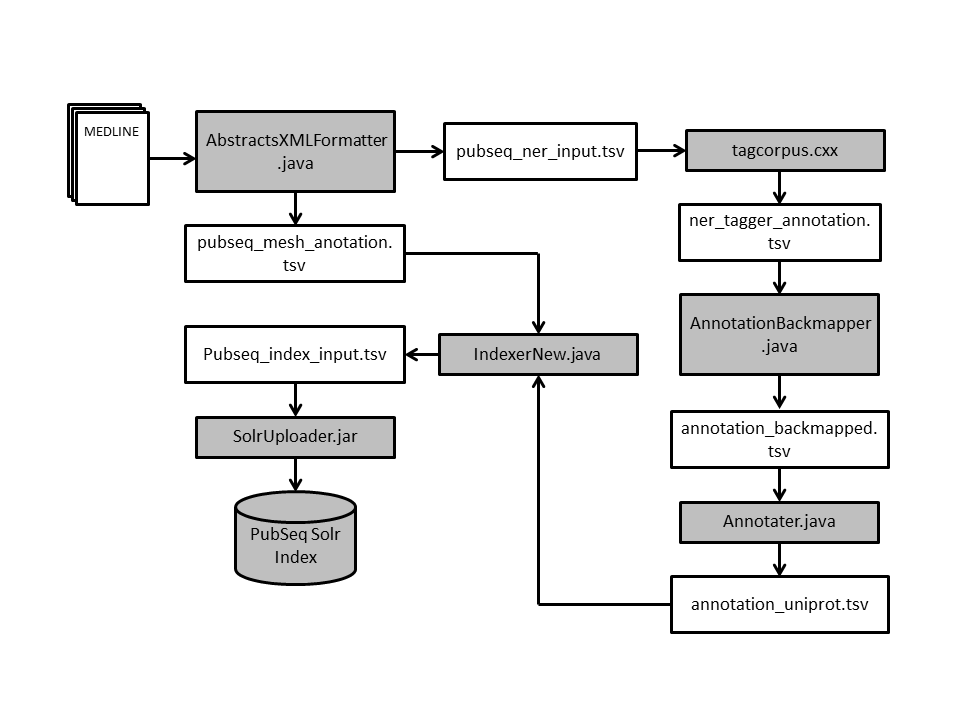
\includegraphics[width=6in]{Figures/tagging_pipeline_complete.png}
    \rule{35em}{0.5pt}
  \caption[(Resized) Overview of PubSeq Tagging Pipeline with all essential programs showed as nodes and important input/output files shown]{Overview of PubSeq Tagging Pipeline. Here we see how the raw data, MEDLINE XML file, is going through layers of program and ends up as input data for Solr Index. Here we also noticed that the workflow is structured as directed acyclic graph, where some data from non-immediate previous step would be used in later steps. The larger, original size of the workflow could be found in Appendix \ref{fig:PubSeqTaggingFull}}
  \label{fig:PubSeqTaggingComplete}
\end{figure}

%----------------------------------------------------------------------------------------
%	SECTION 2
%----------------------------------------------------------------------------------------

\section{MEDLINE Abstracts}

\label{sec:MEDLINEAbstracts}

We used NLM's leasing scheme \citep{MEDLINE} to retrieve the MEDLINE corpus. Each day, an updated from MEDLINE server is downloaded via FTP protocol onto our server. The update will happen daily at around 8 A.M. server time (CET/CEST). Each update is formatted as an XML file, each with an incrementing numerical identifier: the files are named \texttt{meldine15nXXXX.xml} with \texttt{XXXX} the integer identifier -- that is, the update file \texttt{meldine15n1057.xml} comes right after \texttt{meldine15n1056.xml} and before \texttt{meldine15n1058.xml}. The definition of MEDLINE XML file currently follows National Library of Medicine's (NLM) MEDLINE/PubMed Document Type Definition (DTD) \citep{MEDLINEDTD}, which at the time of thesis writing, is currently at the version dated 01/01/2015 \footnote{accessed 8/20/2015}.


Following is a slightly redacted example of a MEDLINE reference, which is taken for the paper by Karapakis-Liaskos and Ferrero, Nat. Rev. Immunol., 2015\footnote{doi:10.1038/nri3837}:

\label{lst:MEDLINEDTD}
\begin{lstlisting}[breaklines]
<MedlineCitation Owner="NLM" Status="In-Data-Review">
<PMID Version="1">25976515</PMID>
<DateCreated>
<Year>2015</Year>
<Month>05</Month>
<Day>26</Day>
</DateCreated>
<Article PubModel="Print-Electronic">
<Journal>
<ISSN IssnType="Electronic">1474-1741</ISSN>
<JournalIssue CitedMedium="Internet">
<Volume>15</Volume>
<Issue>6</Issue>
<PubDate>
<Year>2015</Year>
<Month>Jun</Month>
</PubDate>
</JournalIssue>
<Title>Nature reviews. Immunology</Title>
<ISOAbbreviation>Nat. Rev. Immunol.</ISOAbbreviation>
</Journal>
<ArticleTitle>Immune modulation ... membrane vesicles.</ArticleTitle>
<Pagination>
<MedlinePgn>375-87</MedlinePgn>
</Pagination>
<ELocationID EIdType="doi" ValidYN="Y">10.1038/nri3837</ELocationID>
<Abstract>
<AbstractText>Gram-negative ... nanotechnologies.</AbstractText>
</Abstract>
<AuthorList CompleteYN="Y">
<Author ValidYN="Y">
<LastName>Kaparakis-Liaskos</LastName>
<ForeName>Maria</ForeName>
<Initials>M</Initials>
<AffiliationInfo>
<Affiliation>MIMR-PHI Institute of ..., Australia.</Affiliation>
</AffiliationInfo>
</Author>
<Author ValidYN="Y">
<LastName>Ferrero</LastName>
<ForeName>Richard L</ForeName>
<Initials>RL</Initials>
<AffiliationInfo>
<Affiliation>MIMR-PHI Institute of ..., Australia.</Affiliation>
</AffiliationInfo>
</Author>
</AuthorList>
<Language>eng</Language>
<PublicationTypeList>
<PublicationType UI="D016428">Journal Article</PublicationType>
</PublicationTypeList>
<ArticleDate DateType="Electronic">
<Year>2015</Year>
<Month>05</Month>
<Day>15</Day>
</ArticleDate>
</Article>
<MedlineJournalInfo>
<Country>England</Country>
<MedlineTA>Nat Rev Immunol</MedlineTA>
<NlmUniqueID>101124169</NlmUniqueID>
<ISSNLinking>1474-1733</ISSNLinking>
</MedlineJournalInfo>
<CitationSubset>IM</CitationSubset>
</MedlineCitation>
\end{lstlisting}

%----------------------------------------------------------------------------------------
%	SUBSECTION 2.1
%----------------------------------------------------------------------------------------

\subsection{Specifications}

\begin{table}[htbp]
\caption{Specifications table for PubSeq MEDLINE Abstracts}
\centering
\begin{tabular}{ | l | l | }
  \hline
  Parameter & Value \\
  \hline
  URL, repo & none \\
  Path, clone & none \\
  Path, running program & \texttt{/mnt/project/rost\_db/medline}\\
  \hline
\end{tabular}
\end{table}

%\begin{figure}[!h]
%	\theverbbox
%\caption{An example of a reference from XML MEDLINE corpus}
%\label{fig:singlecell_chemo}
%\end{figure}

%----------------------------------------------------------------------------------------
%	SECTION 3
%----------------------------------------------------------------------------------------

\section{XMLAbstractFormatter.java}

\label{sec:XMLAbstractFormatter}

This class represents a formatter that parses the MEDLINE abstract files and transforms it into STRING Tagger-compliant format. It follows NLM DTD for MEDLINE \citep{MEDLINEDTD} as parsing reference. In the directory where the updates were downloaded, it lists down all possible XML files and parses files that had not been processed before. For each XML file, it creates a tree representation of the file through full. Owning to its tree-like structure \citep{bray2011extensible} \citep{MEDLINEDTD}, this implies that each \texttt{MedlineCitation} tag is itself is a tree (see Section \ref{lst:MEDLINEDTD}) . For each \texttt{MedlineCitation} it extracts needed information such as PubMed ID, title, journal name, publication date, abstract, authors and associated MeSH IDs \citep{lowe1994understanding} and writes it out.

\subsection{Parameters}

\begin{lstlisting}[breaklines]
path_to_medline ner_output_path mesh_output_path counter_file counter_max
\end{lstlisting}

\begin{itemize}
\item \texttt{path\_to\_medline}: the location of MEDLINE xml abstracts. The program will recursively traverse all sub directories of this path and parse files matching following name pattern: \texttt{meldine15nXXXX.xml}.

\item \texttt{ner\_output\_path}: path the first output file (with name) should be written onto. The first output file would then be used for Tagging by PubSeq NER Tagger.

\item \texttt{mesh\_output\_path }: to path the second output file (with name) should be written onto. The second output file contains associative table between PMID and list of MeSH IDs associated with the publication. Since STRING Tagger input is fixed we write this information in separate file.

\item \texttt{counter\_file}: file containing the location of last parsing. The program parses \texttt{XXXX} of the name format and figures whether current integer is larger than the one written in \texttt{counter\_file} before parsing the content of the update file. Upon the completion of the run, the program will replace the value within \texttt{counter\_file} with the largest \texttt{XXX} it encountered. This would be then the starting point of the next run.

\item \texttt{counter\_max}: file containing the maximum \texttt{XXXX} this program should read. If \texttt{counter\_file} contains 1000 and \texttt{counter\_max} 1500 it will only parse \texttt{meldine15n1001.xml} all the way through \texttt{meldine15n1500.xml} in this run. Note that \texttt{counter\_max} is not updated after run. If \texttt{counter\_max} doesn't exist in system then the it assumes \texttt{Integer.MAX\_VALUE} \footnote{\href{http://docs.oracle.com/javase/7/docs/api/java/lang/Integer.html}{\texttt{http://docs.oracle.com/javase/7/docs/api/java/lang/Integer.html}}, accessed 08/20/2015} as upper bound of the parsing.
\end{itemize}

\subsection{Specifications}

\begin{table}[htbp]
\caption{Specifications table for XMLAbstractsFormatter.java}
\centering
\begin{tabularx}{\textwidth}{ | l | X | }
  \hline
  Parameter & Value \\
  \hline
  URL, repo & See Appendix \ref{AppendixA} \\
  Path, clone & \texttt{/mnt/project/pubseq/dev/pubseq-tagging /PubSeq/src/org/pubseq/utils/ XMLAbstractsFormatter.java} \\
  Path, running program & \texttt{/mnt/project/pubseq/dev/pubseq-tagging /PubSeq/src/org/pubseq/utils/ XMLAbstractsFormatter.java} \\
  \hline
\end{tabularx}
\end{table}

%----------------------------------------------------------------------------------------
%	SECTION 4
%----------------------------------------------------------------------------------------

\section{tagcorpus.cxx}

This program is the core component of our Tagging Pipeline. It takes a tab-separated file as input and tags various entities within each abstract. Originally developed by Jensen et al at University of Copenhagen, the backbone of the program is based in NER tagging environment that was used in (Pacifilis, et al, 2013 \citep{pafilis2013species}), which in turn utilizes dictionaries curated within the framework of STRING database (Szklarczyk, et al, 2011 \citep{szklarczyk2011string}).

In very broad explanation, the program uses various kind of mapping for various entities. While parsing a text, the program checks for word combinations that looks similar to the entries that were mapped (i.e. the word has small Levensthein distance \citep{levenshtein1966binary} to some word within the map). For an NER program, the program is astonishingly fast. A full set of MEDLINE corpus with ca. 26 million articles could be parsed in under 12 hours (the mileage may vary according to server specification and number of threads involved).

Our entry point into the program is \texttt{tagcorpus.cxx}. There are several modi of running the program. However, in the modus that we use to tag MEDLINE abstracts, we call the tagger in following manner:


\begin{lstlisting}[breaklines]
input_file | path_to_named_entity_tagger/tagcorpus path_to_pubseq_programdata/entities.tsv path_to_named_entity_tagger_data/names.tsv path_to_named_entity_tagger_data/global.tsv path_to_named_entity_tagger_data/local.tsv path_to_named_entity_tagger_data/groups.tsv > output_file_path
\end{lstlisting}

\begin{itemize}
\item \texttt{input\_file} is the formatted input from \texttt{XMLAbstractsFormatter.java}.
\item \texttt{path\_to\_named\_entity\_tagger/tagcorpus}: the location of compiled binary \texttt{tagcorpus.cxx}, our gateway to the program. See Appendix \ref{AppendixA} for the detail of program structure.
\item \texttt{path\_to\_pubseq\_programdata/entities.tsv}: the location of table \texttt{entities.tsv}.
\item \texttt{path\_to\_pubseq\_programdata/names.tsv}: the location of table \texttt{names.tsv}.
\item \texttt{path\_to\_pubseq\_programdata/global.tsv}: the location of table \texttt{global.tsv}.
\item \texttt{path\_to\_pubseq\_programdata/local.tsv}: the location of table \texttt{local.tsv}.
\item \texttt{path\_to\_pubseq\_programdata/groups.tsv}: the location of table \texttt{groups.tsv}.
\end{itemize}

While there are several input files besides the prepared MEDLINE abstracts file itself, there are only four tables that we are mainly concerned with: the MEDLINE input table itself, \texttt{entities.tsv}, \texttt{names.tsv} and the output table.

\subsection{MEDLINE Input Table}

The NER Tagger takes a tab-separated table with following format as input:

\begin{itemize}
\item first column: PMID of the article with format of \texttt{PMID:article\_pmid}.
\item second column: list of authors. Each author is separated with semicolon.
\item third column: journal name.
\item fourth column: publication date.
\item fifth column: title.
\item sixth column: abstract.
\end{itemize}

Following is an example of valid input line, taken for the paper by Gu, et al, The Journal of Cell Biology, 1999 \footnote{doi: 10.1083/jcb.147.5.1085}:


\begin{lstlisting}[breaklines]
10579727	M Gu;X Xi;G D Englund;M C Berndt;X Du	The Journal of cell biology	1999-11-29T00:00:01Z	Analysis of the roles of 14-3-3 in the platelet glycoprotein Ib-IX-mediated activation of integrin alpha(IIb)beta(3) using a reconstituted mammalian cell expression model.	We have reconstituted the platelet glycoprotein (GP) Ib-IX-mediated activation of the integrin alpha(IIb)beta(3) in a recombinant DNA expression model, and show that 14-3-3 is important in GPIb-IX signaling. CHO cells expressing alpha(IIb)beta(3) adhere poorly to vWF. Cells expressing GPIb-IX adhere to vWF in the presence of botrocetin but spread poorly. Cells coexpressing integrin alpha(IIb)beta(3) and GPIb-IX adhere and spread on vWF, which is inhibited by RGDS peptides and antibodies against alpha(IIb)beta(3). vWF binding to GPIb-IX also activates soluble fibrinogen binding to alpha(IIb)beta(3) indicating that GPIb-IX mediates a cellular signal leading to alpha(IIb)beta(3) activation. Deletion of the 14-3-3-binding site in GPIbalpha inhibited GPIb-IX-mediated fibrinogen binding to alpha(IIb)beta(3) and cell spreading on vWF. Thus, 14-3-3 binding to GPIb-IX is important in GPIb-IX signaling. Expression of a dominant negative 14-3-3 mutant inhibited cell spreading on vWF, suggesting an important role for 14-3-3. Deleting both the 14-3-3 and filamin-binding sites of GPIbalpha induced an endogenous integrin-dependent cell spreading on vWF without requiring alpha(IIb)beta(3), but inhibited vWF-induced fibrinogen binding to alpha(IIb)beta(3). Thus, while different activation mechanisms may be responsible for vWF interaction with different integrins, GPIb-IX-mediated activation of alpha(IIb)beta(3) requires 14-3-3 interaction with GPIbalpha.
\end{lstlisting}

\subsection{entities.tsv}

\texttt{entities.tsv} is a three-column tsv table listing down all unique entity that is taggable by the program. Entity is the smallest unit from speech that is differential from each other. While being the smallest, an entity comes in many forms, with each lexically identifiable with each other. For example, \textit{United States of America}, \textit{America} and \textit{USA} belong to the same entity and are differentiable from \textit{France}, \textit{Republic of France} and \textit{French Republic}, all of which are identifiable with each other and belong to same entity. In STRING Tagger environment, we used STRING ID \citep{szklarczyk2011string} as our identifier \textit{within the Tagger} -- not to be confused with UniProt ID as unique protein identifier in PubSeq system.


Each of three column is defined as follows:


\begin{itemize}
\item first column: the STRING ID of an entity. STRING ID is unique identifier of each entity within STRING Tagger environment. An entity could be understood as one single unique named-entity that is recognizable in text (see explanation bellow).
\item second column: the designation of entity within NCBI Taxonomy Browser \footnote{\href{http://www.ncbi.nlm.nih.gov/taxonomy}{\texttt{http://www.ncbi.nlm.nih.gov/taxonomy}}, accessed 23/08/2015} \citep{federhen2012ncbi}. Since NER Tagger tags various kind of named-entity from protein to disease names, each kind of tag has to be assigned to an identifier describing what kind of named-entity does one entity belong to. A gene/protein belonging to human, for example, will be assigned value of 9606 \footnote{\href{http://www.ncbi.nlm.nih.gov/taxonomy/?term=9606}{\texttt{http://www.ncbi.nlm.nih.gov/taxonomy/?term=9606}}, accessed 23/08/2015}.
\item third column: the representation of this entity in alphanumeric form. The name which appears in this entry would be referred as \textbf{standard name} in later parts.
\end{itemize}

As explained before, a single entity could map to multiple written values. This mapping is described in another table, \texttt{names.tsv}.

\subsection{names.tsv}

\texttt{names.tsv} is mapping table between STRING ID (see the definition for \texttt{entites.tsv} above) and all its written forms. There are two columns in this table:

\begin{itemize}
\item first column: the STRING ID.
\item second column: the name of the entity.
\end{itemize}

As expected, the relation of this table is \textbf{1 x N}, that is, each of the element on the right is associated with only one element of the right and each of the elements on the left is associate with N elements on the right. Also, for each String ID from table entities.tsv, the entry from the third column of the table is also contained in \texttt{names.tsv}.

\subsection{STRING Tagger Annotation}

After finishing the tagging process, the NER Tagger would produce a file that lists down all annotations that it found. The output file is tab-separated, with each row representing a single annotation. There are 8 columns in the table:

\begin{itemize}
\item first column defines the PMID on which this annotation is found.
\item second column defines the start of internal ordering of annotation within STRING Tagger.
\item third column defines the end of internal ordering of annotation within STRING Tagger.
\item fourth column defines the start offset of the annotation within the input text.
\item fifth column defines the end offset of the annotation within the input text, inclusive.
\item sixth column defines tagged string as it appears in the input text.
\item seventh column defines designated associated taxonomy of entities the string is annotated with (see second column of \texttt{entities.tsv}).
\item eighth column defines the STRING ID of the entity the string is annotated with (see first column of \texttt{entities.tsv}.
\end{itemize}

As expected, the eight and ninth columns of the output file are coupled. Note also that a string within input text could be annotated with multiple entities. The reason for this is because since the string found in input text is likely to be ambiguous and has therefore to be tagged with multiple entities. To take as an example, \textit{America} could mean both \textit{United States of America} and the continent. Also given the enormous size of entities within \texttt{entities.tsv}, combinatorically the likelihood that two entities posses very similar written forms could not be trivialized.

%----------------------------------------------------------------------------------------
%	SECTION 5
%----------------------------------------------------------------------------------------

\section{AnnotationBackmapper.java}

\label{sec:AnnotationBackmapper}

This class modifies the results from STRING Tagger. The program AnnotationBackmapper.java does following task:

\begin{itemize}
\item Backmapping of the annotations (see bellow).
\item Computing statistics of the number of articles with annotation and the number of annotations. Note that the annotations taken statistics of include all possible kind of annotations that the NER tagging done (i.e. not only protein annotation)
\end{itemize}

The main task of this program is to map the sixth column of each of the NER Tagger annotations back to the name as it appears in entities.tsv. That is, given a result:

\begin{verbatim}
12345	1	1	11	13	some annotation	9606	23456789
\end{verbatim}

and the entry of \texttt{23456789} within \texttt{entities.tsv}:

\begin{verbatim}
23456789	9606	standard name
\end{verbatim}

this program replaces \texttt{some annotation} with \texttt{standard name}:

\begin{verbatim}
12345	1	1	11	13	standard name	9606	23456789
\end{verbatim}

This mapped back would be used in later part of the Tagging Process. Also knowing the standard name would help in development process and sanity check, since standard name is usually (in case of protein) unique within some databases (for example, most proteins have ENSEMBL ID as its standard name), albeit not uniformly -- the identifiers hailed from various systems including ENSEBML \citep{hubbard2002ensembl}, VectorBase \citep{lawson2009vectorbase} and some even have ordered locus (OLS) name as identifier \footnote{\href{http://www.uniprot.org/help/gene_name}{\texttt{http://www.uniprot.org/help/gene\_name}}, accessed 23/08/2015}.

\subsection{Parameters}

\begin{lstlisting}[breaklines]
ner_annotations entities_table result_path statistics_path
\end{lstlisting}

\begin{itemize}
\item \texttt{ner\_annotations}: the result of STRING Tagger.
\item \texttt{entities\_table}: the table as appeared in STRING Tagger.
\item \texttt{results\_path}: the path the backmapped annotations are to be written to.
\item \texttt{statistics\_path}: the file the statistics is to be written to.
\end{itemize}

\subsection{Specifications}

\begin{table}[htbp]
\caption{Specifications table for AnnotationBackmapper.java}
\centering
\begin{tabularx}{\textwidth}{ | l | X | }
  \hline
  Parameter & Value \\
  \hline
  URL, repo & See Appendix \ref{AppendixA} \\
  Path, clone & \texttt{/mnt/project/pubseq/pandu/pubseq-crawler/PubSeq /src/org/pubseq/annotation /AnnotationBackmapper.java} \\
  Path, running program & \texttt{/mnt/project/pubseq/pandu/pubseq-crawler/PubSeq /src/org/pubseq/annotation /AnnotationBackmapper.class}\\
  \hline
\end{tabularx}
\end{table}

%----------------------------------------------------------------------------------------
%	SECTION 6
%----------------------------------------------------------------------------------------

\section{Annotater.java}

This program "annotates" the tagging results of the NER tagger. Given a result row from NER Tagger, it checks whether the annotation is protein annotation -- if so, it then tries to find all UniProt IDs that this annotation maps to. As described before, every single annotation from NER tagger is associated with STRING ID and each STRING ID is described in \texttt{entities.tsv} with a standard name. This is also the case for protein annotation, it is associated with some identifier as standard name. The identifiers used are, however, not strucrtured and belong to single identifying system such as UniProt ID or ENSEMBL (see Section \ref{sec:AnnotationBackmapper}). This might seem problematic as the start since we decided to only use UniProt ID as standard and unique identifier for proteins. The NER Tagger however, provides such mapping implicitly. As explained in previous chapters, the table \texttt{names.tsv} maps each String ID to list of names it is associated with. Within the context of protein entity, each of the STRING ID maps to various names and other identifiers associated with this STRING ID, among others the UniProt IDs. We therefore had to merged these two tables with regard to the String ID and create a new table that maps standard name (that is, name that appears with STRING ID within table \texttt{entities.tsv} to other names that are associated with the same STRING ID. This step fortunately has been done in other step and belongs to the Maintenance Pipeline.

As thus, the program only has to parse the resulting merged table from the Maintenance Pipeline and maps the sixth column (already in standard name, see Section \ref{sec:AnnotationBackmapper}) to the list of all associated names. For each of associated names, an entry is written to output file in format similar to the output format of NER tagger with the sixth column replaced with associated names. That is, for each backmapped annotation from previous step:

\begin{verbatim}
12345	1	1	11	13	standard name	9606	23456789
\end{verbatim}

we checked whether standard name is a UniProt ID. If so, then we write this to output file. Otherwise we check whether there exists some mapping from standard name to list of names within the merged files. If there is one, write for each values the same entry with sixth column replaced:

\begin{verbatim}
12345	1	1	11	13	uniprot_id_1	9606	23456789
...
12345	1	1	11	13	uniprot_id_m	9606	23456789
\end{verbatim}


The multiple mapping of standard name to multiple UniProt IDs could be explained best by the fact that named-entity tagging is prone with lexical ambiguity \citep{ratinov2009design}. A protein named X might have associated with several entries in UniProt database, each with exact or almost exact assigned name. This is especially true in case of unreviewed proteins. There are for example several cases of UniProt entry named \textit{Brain-derived neurotrophic factor} (BNDF) \footnote{\href{http://www.uniprot.org/uniprot/?query=Brain-derived+neurotrophic+factor&sort=score}{\texttt{http://www.uniprot.org/uniprot/?query=Brain-derived+neurotrophic+factor\&sort=score}}, accessed 23/08/2015}. All aforementioned entries are both lexically and ideolexically the same -- they represent very similar things that have very similar name, which would be very hard to disambiguate \citep{ratinov2009design}. This is moreover exacerbated by the fact that many unreviewed proteins have names that are similar or exactly similar to the to the ones that are already reviewed. Looking at context around the annotation location might help to determine whether a named-entity belong to protein or not or whether a tagged protein name belongs to human or not (for example, by looking at whether the sentence/paragraph/paper delves into human disaese etc), however, exactly named protein belonging to same species is hard to differentiate by looking at text. Therefore the multiple mapping.

\subsection{Parameters}

\begin{lstlisting}[breaklines]
ner_backmapped_annotation merged_table uniprot_kbid output_file
\end{lstlisting}

\begin{itemize}
\item \texttt{ner\_backmapped\_annotation}: the result of previous step
\item \texttt{merged\_table}: the merged-filtered table created from \texttt{entities.tsv} and \texttt{names.tsv} (see program description above).
\item \texttt{uniprot\_kbid}: the mapper between UniProt Accession ID and its associated UniProtKB ID \footnote{ \href{ftp://ftp.uniprot.org/pub/databases/uniprot/current_release/knowledgebase/idmapping/}{\texttt{ftp://ftp.uniprot.org/pub/databases/uniprot/current\_release/knowledgebase/idmapping/}}, accessed 23/08/2015}. We use this as a reference for the full list of existing UniProt ID.
\end{itemize}

\subsection{Specifications}

\begin{table}[htbp]
\caption{Specifications table for Annotater.java}
\centering
\begin{tabularx}{\textwidth}{ | l | X | }
  \hline
  Parameter & Value \\
  \hline
  URL, repo & See Appendix \ref{AppendixA} \\
  Path, clone & \texttt{/mnt/project/pubseq/pandu/pubseq-crawler/PubSeq /src/org/pubseq/annotation/Annotater.java} \\
  Path, running program & \texttt{/mnt/project/pubseq/pandu/pubseq-crawler/PubSeq /src/org/pubseq/annotation/Annotater.class}\\
  \hline
\end{tabularx}
\end{table}

%----------------------------------------------------------------------------------------
%	SECTION 7
%----------------------------------------------------------------------------------------

\section{StatisticsUtils.java}


This step is mostly deprecated but is still connected with other program. It was initially intended as statistics mechanism that produces some descriptive statistics on the landscape of annotation for the whole MEDLINE abstract. Since the Tagging Pipeline is done regularly now, this method is not necessary for the whole pipeline.

\subsection{Specifications}

\begin{table}[htbp]
\caption{Specifications table for StatisticsUtils.java}
\centering
\begin{tabularx}{\textwidth}{ | l | X | }
  \hline
  Parameter & Value \\
  \hline
  URL, repo & See Appendix \ref{AppendixA} \\
  Path, clone & \texttt{/mnt/project/pubseq/pandu/pubseq-crawler/PubSeq /src/org/pubseq/utils/StatisticsUtils.java} \\
  Path, running program & \texttt{/mnt/project/pubseq/pandu/pubseq-crawler/PubSeq /src/org/pubseq/utils/StatisticsUtils.class}\\
  \hline
\end{tabularx}
\end{table}

%----------------------------------------------------------------------------------------
%	SECTION 8
%----------------------------------------------------------------------------------------

\section{IndexerNew.java}

\texttt{IndexerNew.java} is the last step before pushing the input data onto Solr index. The main purpose of this step is to put all information that were acquired during the Tagging Pipeline together. There are three kinds of information that we are particularly interested in form our pipeline:

\begin{itemize}
\item List of proteins that are mentioned in an article
\item List of taxonomy association of the proteins in the article
\item List of MeSH IDs of the article
\end{itemize}

The first information was obtained during NER Tagging process, while the latter two were obtained while parsing raw MEDLINE XML input. We will use the initially formatted MEDLINE file (see Section \ref{sec:XMLAbstractFormatter} bellow) as the template. The three kinds of information will each occupy one new column in the updated file. Hence, there would be then nine columns in the output file:

\begin{itemize}
\item first column: PMID of the article. Unlike the output format of \texttt{XMLAbstractFormatter.java}, the PMID will appear in plain ID form without the prefix \texttt{PMID:}).
\item second column: list of authors. Each author is separated with semicolon.
\item third column: journal name as appeared in XML input file.
\item fourth column: publication date.
\item fifth column: article title.
\item sixth column: article abstract. Multi-abstracts (i.e. abstracts with sub-organizations such as introduction, methods, results etc) would be represtented as one string.
\item seventh column: list of UniProt ID mentions, separated by space.
\item eight column: list of MeshID associated with the article, separated by space.
\item ninth column: unique list of UniProt ID species associations, separated by space.
\end{itemize}

To achieve, this, we initialized a map for each of the information, with PMIDs as key and the list of UniProt IDs/unique species/MeSH IDs as value. We do this by simply parsing the results from previous steps that contain the information we'd like to index:

\begin{itemize}
\item \textbf{List of UniProt ID Mentions} are available from post-processed NER tagger annotations. We use the output of Annotater.java. The program implements the index as Hash Map with PMID as key and list of UniProt as values. The file will be parsed sequentially and the UniProt ID annotation (sixth column) for the PMID (first column) would be pushed into the map. At the end, a temporary file will be written with added column created from this index. Upon embedding the merging will done and the result written. Afterwards, the map is deleted to free up memory.
\item \textbf{List of MeSH IDs} are available from \texttt{XMLAbstractFormatter.java}. Since the file is already in form of implicit map (two columns with first column containing PMID and second list of MeSH), the program just parses the file sequentially into the index. The later steps follow roughly the one for UniProt ID mentions.
\item \textbf{List of Species Associations} are available from post-processed NER tagger annotation. As reader can see in the output format of PubSeq NER Tagger, the seventh column contains the taxonomy association of the annotation. As such, this step follows closely the first procedure (List of UniProt ID mentions). The only different would be that the parser uses seventh instead of sixth column as value.
\end{itemize}

he reason behind doing this sequentially is, again, memory. In the worst case when the program has to index the whole MEDLINE abstract, memory usage for each of the step easily exceeds 20 GB. As such sequential steps were used instead of all-in-one approach.

\subsection{Parameters}

\begin{lstlisting}[breaklines]
template_path template_index_col_num output_dir_path first_file_path first_file_index_col_num first_file_value_col_num second_file_path second_file_index_col_num second_file_value_col_num third_file_path third_file_index_col_num third_file_value_col_num final_name
\end{lstlisting}

\begin{itemize}
\item \texttt{template\_path}: path to template file.
\item \texttt{template\_index\_col\_num}: column number of template file's reference column (PMID). This will be used for embedding template with additional columns.
\item \texttt{output\_dir\_path}: the directory where interim and final values are to be stored.
\end{itemize}

For each of the three files:

\begin{itemize}
\item \texttt{path}: output file path.
\item \texttt{index\_col\_num}: column number of the file's reference column (PMID).
\item \texttt{value\_col\_num}: column number of the file's value.
\end{itemize}

Also,

\begin{itemize}
\item \texttt{final\_name}: final name of the output file.
\end{itemize}

\subsection{Specifications}

\begin{table}[htbp]
\caption{Specifications table for IndexerNew.java}
\centering
\begin{tabularx}{\textwidth}{ | l | X | }
  \hline
  Parameter & Value \\
  \hline
  URL, repo & See Appendix \ref{AppendixA} \\
  Path, clone & \texttt{/mnt/project/pubseq/pandu/pubseq-crawler/PubSeq /src/org/pubseq/utils/IndexerNew.java} \\
  Path, running program & \texttt{/mnt/project/pubseq/pandu/pubseq-crawler/PubSeq /src/org/pubseq/utils/IndexerNew.class}\\
  \hline
\end{tabularx}
\end{table}

%----------------------------------------------------------------------------------------
%	SECTION 9
%----------------------------------------------------------------------------------------

\section{IndexerNew.java}

The class from which SolrUpdater.jar derives from, \textbf{SolrUpdater.java}, consists of module that will push new documents (Solr term for an entry) onto the index. Given the input table with updated columns from IndexerNew.java, this programs parses and pushes each row from the input. For each row from the input, the program checks whether such document already exists in the Solr index. If such document exists, it updates the attributes of existing document by adding new values coming from the parsed row. Otherwise, the program creates a document instance containing the values from parsed row as attributes. The document instance would then be pushed onto the index. The whole process utilizes the Solr native API for Java, SolrJ \citep{grainger2014solr} \footnote{\href{https://wiki.apache.org/solr/Solrj}{\texttt{https://wiki.apache.org/solr/Solrj}}, accessed 23/08/2015} \footnote{\href{https://cwiki.apache.org/confluence/display/solr/Using+SolrJ}{\texttt{https://cwiki.apache.org/confluence/display/solr/Using+SolrJ}}, accessed 23/08/2015}.

\subsection{Parameters}

\begin{lstlisting}[breaklines]
abstract_output_path index_url
\end{lstlisting}

\begin{itemize}
\item \texttt{abstract\_output\_path}: path of directory containing input table.
\item \texttt{index\_url}: URL on which the PubSeq core is accessible from see Chapter \ref{Chapter5} for the description of core within Solr environment. The URL of a core within an environment is basically a subpage of the index itself. That is, for an index located at \texttt{http://localhost:8983/solr/}, the address of core named \texttt{pubseq} would be \texttt{http://localhost:8983/solr/pubseq/}.
\end{itemize}

\subsection{Specifications}

\begin{table}[htbp]
\caption{Specifications table for SolrUploader.java}
\centering
\begin{tabularx}{\textwidth}{ | l | X | }
  \hline
  Parameter & Value \\
  \hline
  URL, repo & See Appendix \ref{AppendixA} \\
  Path, clone & \texttt{/mnt/project/pubseq/pandu/pubseq-crawler/PubSeq /src/org/pubseq/utils/SolrUploader.java} \\
  Path, running program & \texttt{/mnt/project/pubseq/pandu/pubseq-crawler/PubSeq /SolrUploader.jar}\\
  \hline
\end{tabularx}
\end{table} 
% Chapter Template

\chapter{PubSeq Solr Index} % Main chapter title

\label{Chapter5} % Change X to a consecutive number; for referencing this chapter elsewhere, use \ref{ChapterX}

\lhead{Chapter 5. \emph{PubSeq Solr Index}} % Change X to a consecutive number; this is for the header on each page - perhaps a shortened title

This chapter tries to answer the second question posed in Section \ref{sec:Chap3Intro}: \textit{how the data is going to be stored?} We would see the reason behind our choice of storage technology. We would then also try to specify the definition of our index.

%----------------------------------------------------------------------------------------
%	SECTION 1
%----------------------------------------------------------------------------------------

\section{Solr: Fast and Scalable Indexing}

Apache Solr is an open source enterprise search platform. Initially developed by Yonik Seeley at CNET Networks, it was later published as open source through donation to Apache Software Foundation \footnote{\href{https://issues.apache.org/jira/browse/SOLR-1}{\texttt{https://issues.apache.org/jira/browse/SOLR-1}}, accessed 25/08/2015}. The system is based on Lucene internally, which implements the indexing routine and mechanism \citep{hatcher2004lucene}.

Unlike SQL based system which uses tabular data representation as underlying data storage mechanism, Solr utilizes indexing mechanism in its system \citep{smiley2015apache}. This non-SQL characteristics of data storage and maintenance are generally known as NoSQL. (Brewer, 2000) \citep{brewer2000towards} did some nice overview of comparison between NoSQL and conventional SQL, which could be seen on Table \ref{fig:ACIDvsBASE}

\begin{table}[htbp]
\caption{ACID vs. BASE database property models. ACID vs. BASE database property models. Some NoSQL databases implement ACID, others do not. Taken from (Wachinger, 2013) \citep{wachinger2013next}, adopted from (Brewer, 2000) \citep{brewer2000towards}.}
\begin{tabularx}{\textwidth}{ | l | X | }
  \hline
  ACID (relational model) & BASE (NoSQL) \\
  \hline
  Atomicity, Consistency, Isolation, Durability & Basically Available, Soft state, Eventually consistent \\
  Isolation & Availability First \\
  Focus on Commit & Best Effort \\
  Nested Transactions & Approximative Answers Acceptable \\
  Non-quaranteed Availability & Aggressive (Optimistic) \\
  Conservative (pessimistic) & Simpler \\
  Difficult Evolution (schema) & Faster, Easier Evolution \\
  \hline
\end{tabularx}
  \label{fig:ACIDvsBASE}
\end{table}

While most NoSQL implementations don't strictly follow ACID criterions, most don't fall into BASE category either. Also, many NoSQL implementations focus on particular use case rather than aim at general data storage purpose. In this regard, Solr aims to be able to store and index in the order of millions and billions documents while optimizing for -- among others -- faceted search \citep{tunkelang2009faceted}, string search and result paging\footnote{\href{https://cwiki.apache.org/confluence/display/solr/Pagination+of+Results}{\texttt{https://cwiki.apache.org/confluence/display/solr/Pagination+of+Results}}, accessed 24/05/2015}. Solr also supports implicit definition of text syntax through definition of stopping sign, language rules etc -- this malleability is used for example, for Solr to be able to optimize for specific language it indexes \citep{grainger2014solr}. This way, Solr not only stores the data efficiently but in a way understand the logic of the data.

Formally, we define our reason of using Solr as follows:

\begin{itemize}
\item \textbf{Reverse indexing}. Possibly the strongest proposition of using Solr, reverse indexing refers to listing down \textit{where in which documents does a string appears in the index}, instead of \textit{which strings appear in which document in the index} \ref{fig:SolrReverseIndexing}. This reverse paradigm enables Solr to retrieve string related queries in almost constant time \citep{grainger2014solr}.
\item \textbf{Automatic Query Weighting}. In its query syntax, Solr enables weighted string matching query. Take for example following content of Solr query: 
\begin{center}
\texttt{unirotid:P53\_HUMAN\textasciicircum2 AND uniprotid:P53\_HORSE}
\end{center}
In this query, \texttt{unirotid:P53\_HUMAN} would be given twice as much weight as \texttt{uniprotid:P53\_HORSE}. For complex analysis involving multiple string queries this proves to be a powerful feature.
\item \textbf{Easy Deployment}. Each unpacked Solr directory could be run to create an instance of server. The only external requirement for Solr is installed Java Virtual Machine (JVM). This makes easier for us for example to test our index in various environment, therefore reducing iteration overhead.
\item \textbf{Native Java Implementation}. Combined with its native Java API, SolrJ, it ensures easier interaction and development of the index.
\item \textbf{Result Pagination}. Solr natively supports results pagination\footnote{\href{https://cwiki.apache.org/confluence/display/solr/Pagination+of+Results}{\texttt{https://cwiki.apache.org/confluence/display/solr/Pagination+of+Results}}, accessed 25/08/2015}. This means that, for very huge query result the system doesn't have to dump the whole result in memory. For our specific purpose, this proves helpful.
\end{itemize}

\begin{figure}[htbp]
    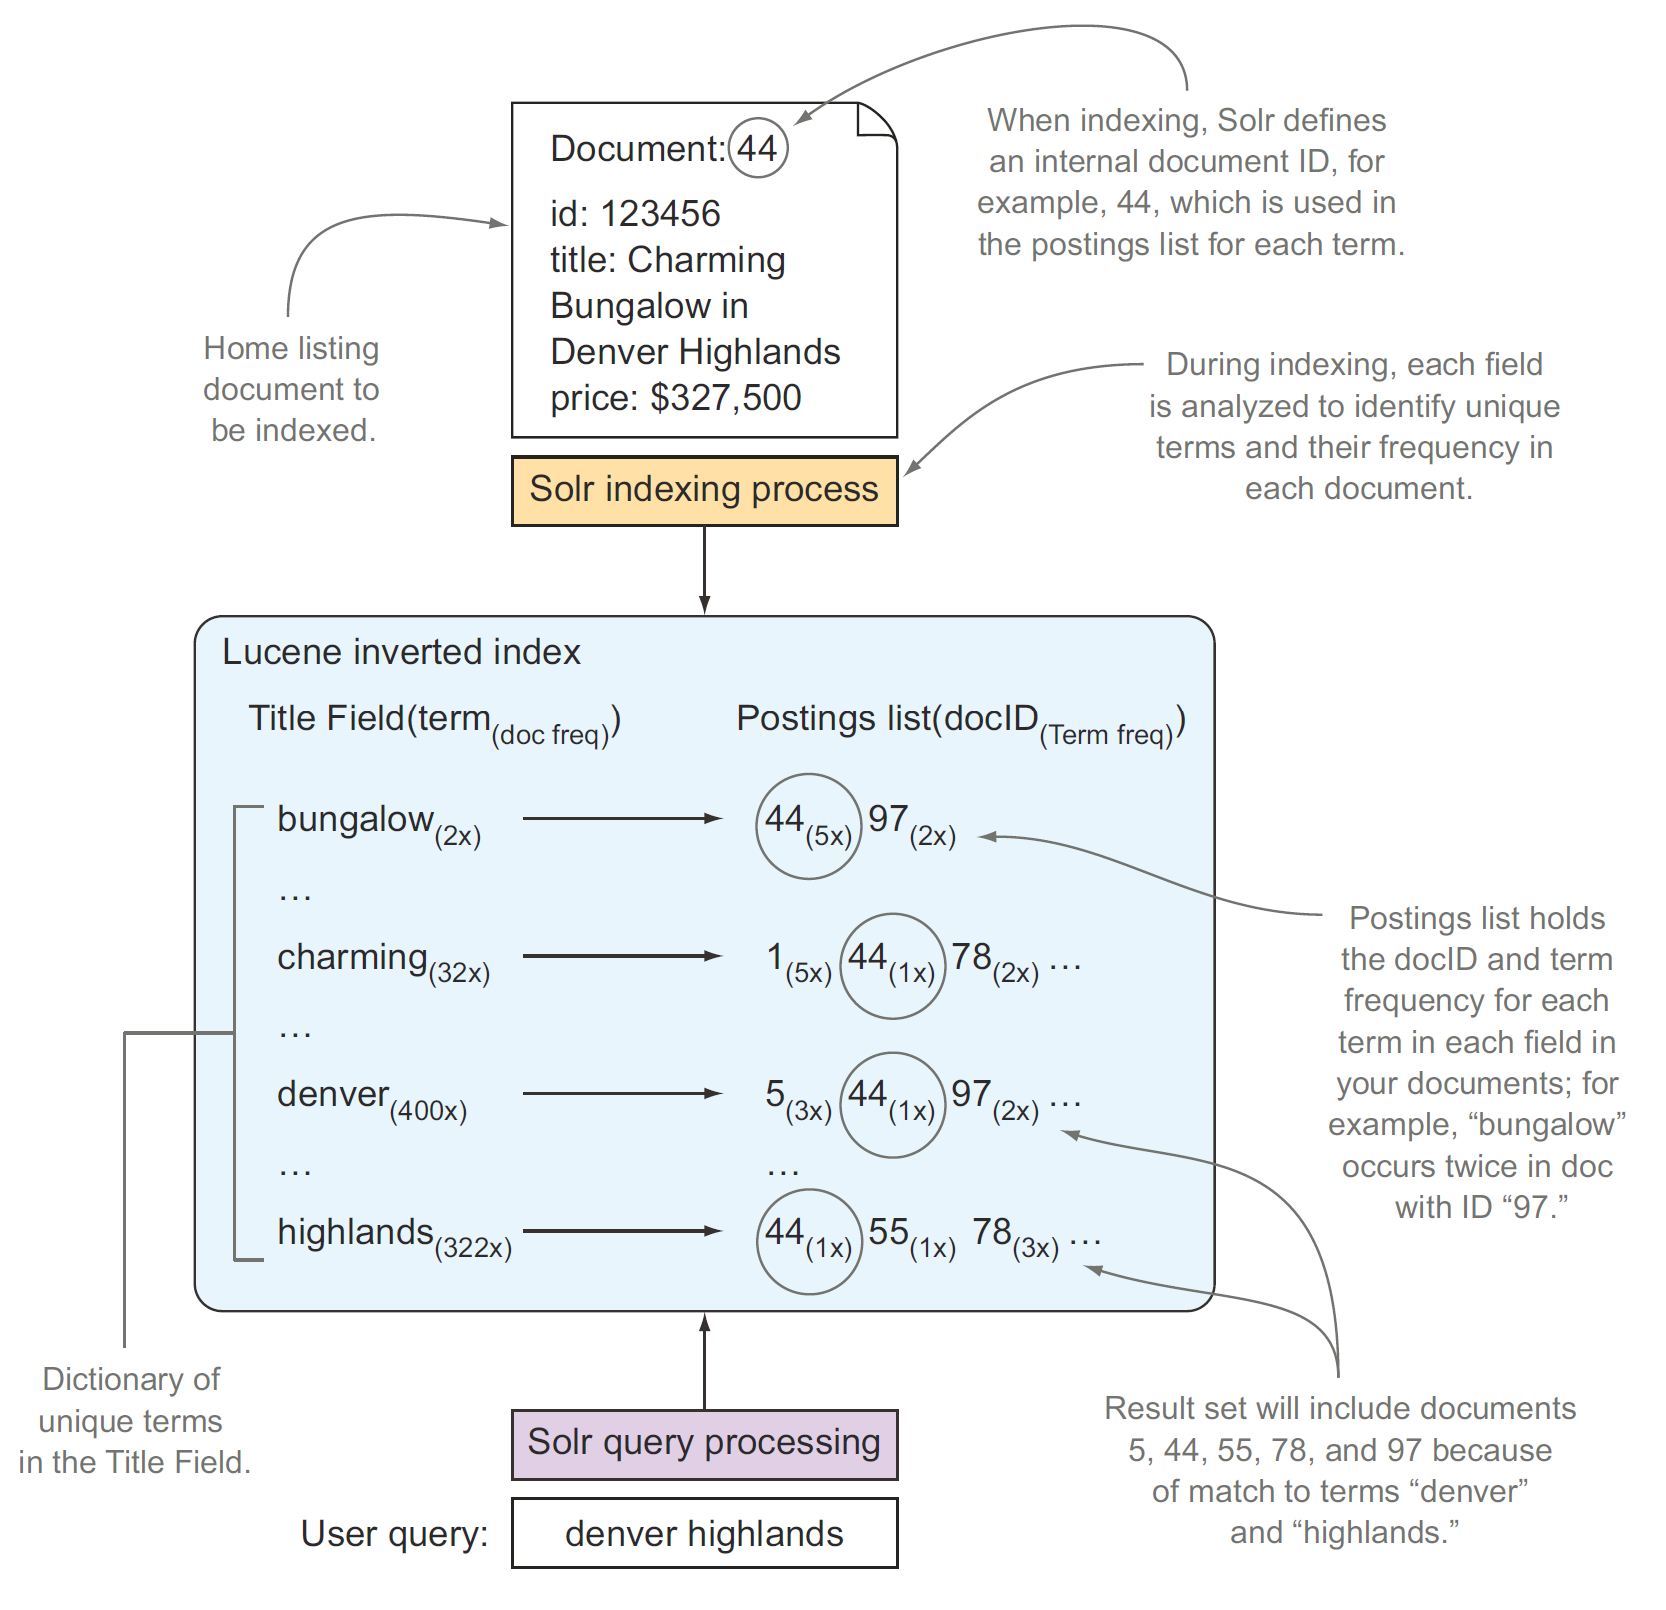
\includegraphics[width=6in]{Figures/solr_reverse_indexing.png}
    \rule{35em}{0.5pt}
  \caption[The key data structure supporting information retrieval is the inverted index within Solr system.]{Overview of reverse indexing mechanism employed by Solr. Here we see how a document is being parsed and represented internally within the mapping of tokens. Beyond Solr, reverese indexing is powerful tool in the field of Information Retrieval (IR) which enables finding occurrences in much reduced time \citep{manning2008introduction}. The fundamentals of reverse indexing in IR follows roughly the same concepts of Solr's reverse indexing. Figure adopted from (Grainger, Potter and Seeley, 2014 \citep{grainger2014solr})}
  \label{fig:SolrReverseIndexing}
\end{figure}

\begin{figure}[htbp]
    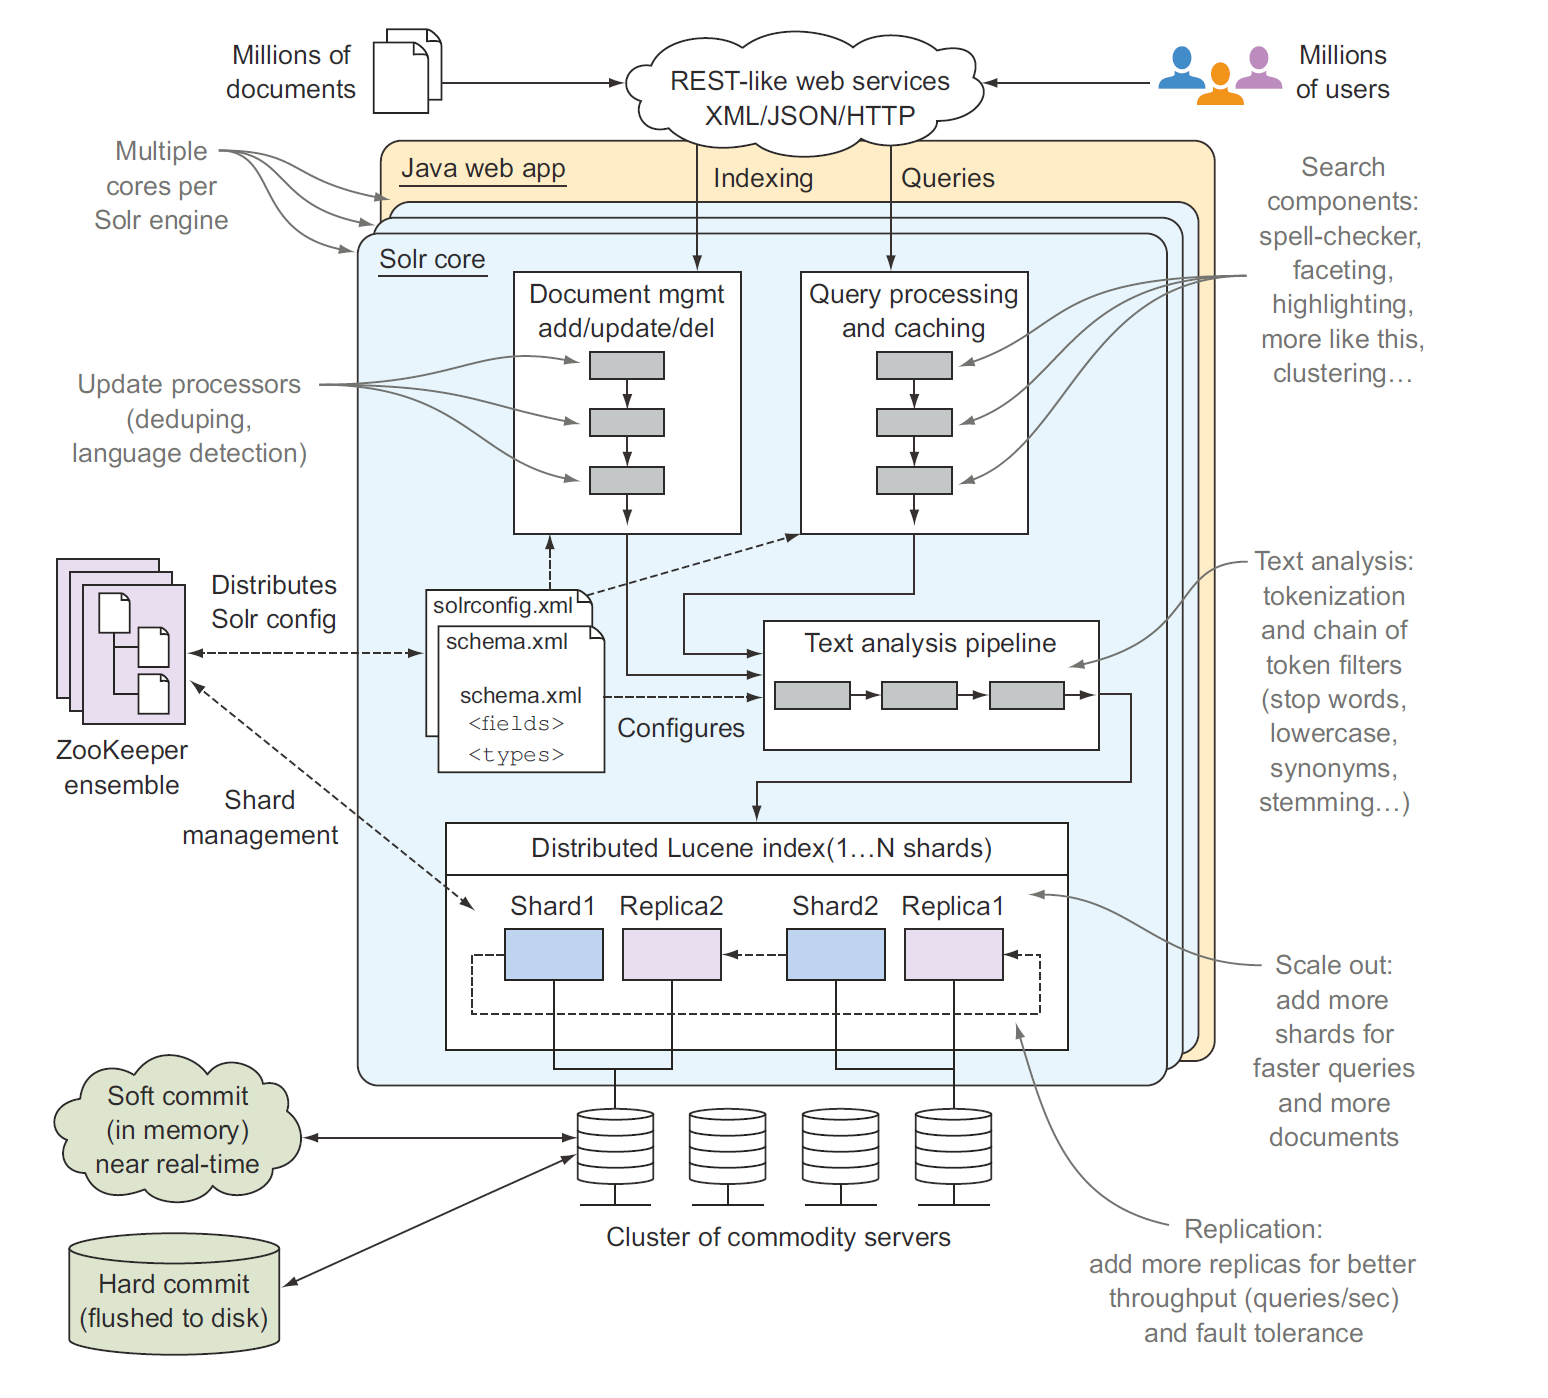
\includegraphics[width=6in]{Figures/solr_components.png}
    \rule{35em}{0.5pt}
  \caption[Diagram of the main components of Solr.]{Diagram of the main components of Solr. There are two main modes of index access: query and indexing. Both modes are handled by the top level REST-like service (wrapped in Jetty \citep{jetty}, Tomcat \citep{apachetomcat} or something similar). Each instance consists of multiple core, with each core is defined by configuration files, namely \texttt{solrconfig.xml} (which applies globally across all cores) and \texttt{schema.xml}. Both indexing and query routines would be going through text analysis pipeline for tokenization and other lexical analysis. Solr would then store/fetch several meta-information in/from appropriate Lucene index. Figure adopted from (Grainger, Potter and Seeley, 2014 \citep{grainger2014solr})}
  \label{fig:SolrComponents}
\end{figure}


There are also other reasons for deploying Solr such as generally lower schema definition complexity, generally powerful syntax etc., which makes even more case for using Solr over other both SQL and non-SQL systems.

%----------------------------------------------------------------------------------------
%	SECTION 2
%----------------------------------------------------------------------------------------

\section{Index Definitions}

Each Solr engine consists of several \textbf{cores} (see Figure \ref{fig:SolrComponents}). Solr wiki page wrote following regarding Solr Core \footnote{\href{https://wiki.apache.org/solr/SolrTerminology}{\texttt{https://wiki.apache.org/solr/SolrTerminology}}, accessed 25/08/2015}:

``
\textit{Solr Core: Also referred to as just a "Core". This is a running instance of a Lucene index along with all the Solr configuration (\texttt{SolrConfigXml}, \texttt{SchemaXml}, etc...) required to use it. A single Solr application can contain 0 or more cores which are run largely in isolation but can communicate with each other if necessary via the \texttt{CoreContainer}. From a historical perspective: Solr initially only supported one index, and the \texttt{SolrCore} class was a singleton for coordinating the low-level functionality at the "core" of Solr. When support was added for creating and managing multiple Cores on the fly, the class was refactored to no longer be a Singleton, but the name stuck.} 
``

Needless to say, Solr core is the lowest abstraction that is configurable within Solr environment. Each Solr core is defined by its own schema. In the mode we were running our Solr on\footnote{Depending on which Solr one is running, a schema could be defined either by \texttt{schema.xml} file or through Schema API (see here: \href{https://cwiki.apache.org/confluence/display/solr/Schema+API}{\texttt{https://cwiki.apache.org/confluence/display/solr/Schema+API}}, accessed 25/08/2015). Both interfaces trigger approximately the same configuration internally.}, we utilize \texttt{schema.xml} to define our schema. For someone more familiar in SQL-based lingo, a core could be thought analogously as table and schema its definition. This definition only works so far since communicating between two cores within Solr is not as trivial as it would be the case for tables in SQL environment.

Similar to SQL fashion, one of the most important aspect of schema definition within Solr is fields definition. We first define our fields in following table:

\begin{table}[htbp]
\caption{Fields definition table for \texttt{pubseq} index within the Solr system.}
\centering
\begin{tabular}{| l | c | c | c | c | c |}
  \hline
  name & type & indexed & stored & required & multiValued \\
  \hline
  \hline
  title & text\_general & \texttt{True} & \texttt{True} & \texttt{True} & \texttt{False} \\
  \hline
  abstract & text\_general & \texttt{True} & \texttt{True} & \texttt{False} & \texttt{False} \\
  \hline
  authors & text\_general & \texttt{True} & \texttt{True} & \texttt{False} & \texttt{True} \\
  \hline
  journal & text\_general & \texttt{True} & \texttt{True} & \texttt{True} & \texttt{False} \\
  \hline
  uniprotid & text\_general & \texttt{True} & \texttt{True} & \texttt{False} & \texttt{True} \\
  \hline
  speceisid & text\_general & \texttt{True} & \texttt{True} & \texttt{False} & \texttt{True} \\
  \hline
  meshid & text\_general & \texttt{True} & \texttt{True} & \texttt{False} & \texttt{True} \\
  \hline
\end{tabular}
  \label{fig:ACIDvsBASE}
\end{table}

\textbf{type} refers to what kind of Java class this field implements. If \textbf{indexed} is true, the value of the field can be used in queries to retrieve matching documents. If \textbf{stored} is true, the actual value of the field can be retrieved by queries. if \textbf{required} is true, the core instructs Solr to reject any attempts to add a document which does not have a value for this field. If \textbf{multiValued} is true, it indicates that a single document might contain multiple values for this field type\footnote{\href{https://cwiki.apache.org/confluence/display/solr/Defining+Fields}{\texttt{https://cwiki.apache.org/confluence/display/solr/Defining+Fields}}, accessed 25/08/2015}. Each multi-valued entry is represented as list internally. This could be invoked using any class implementing List interface \footnote{\href{http://docs.oracle.com/javase/7/docs/api/java/util/List.html}{\texttt{http://docs.oracle.com/javase/7/docs/api/java/util/List.html}}, accessed 25-08-2015}. As query result, depending on the return format (XML, JSON or CSV), this would be returned as either XML list, JSON list oobject or CSV cell-internal list respectively.

Upon creatoin of core, this configuration would be internalized via \texttt{schema.xml}. An example of instance of \texttt{schema.xml} can be found in Appendix \ref{sec:SchemaXMLPath}.

Following is a slightly abridged example of a document within Solr, which is taken for the paper by Takahashi and Yamanaka, Cell, 2006\footnote{doi: 10.1016/j.cell.2006.07.024}:

\label{lst:SolrDoc}
\begin{lstlisting}[breaklines]
{
	"pmid":"16904174",
	"authors":["Kazutoshi Takahashi", "Shinya Yamanaka"],
	"journal":"Cell",
	"pubdate":"2006-08-25T00:00:01Z",
	"title":"Induction of pluripotent stem cells from mouse embryonic and adult fibroblast cultures by defined factors.",
	"abstract":"Differentiated cells can be reprogrammed to an embryonic-like state by transfer of nuclear contents into oocytes or by fusion with embryonic stem (ES) cells. Little is known about factors that induce this reprogramming. Here, we demonstrate induction of pluripotent stem cells from mouse embryonic or adult fibroblasts by introducing four factors, Oct3/4, Sox2, c-Myc, and Klf4, under ES cell culture conditions. Unexpectedly, Nanog was dispensable. These cells, which we designated iPS (induced pluripotent stem) cells, exhibit the morphology and growth properties of ES cells and express ES cell marker genes. Subcutaneous transplantation of iPS cells into nude mice resulted in tumors containing a variety of tissues from all three germ layers. Following injection into blastocysts, iPS cells contributed to mouse embryonic development. These data demonstrate that pluripotent stem cells can be directly generated from fibroblast cultures by the addition of only a few defined factors.",
	"uniprotid":["B3CJ88_HUMAN", "B3CJC0_HUMAN", "Q3V2B6_MOUSE", "B3CJ65_HUMAN", "A2RS90_MOUSE", "B3CJB3_HUMAN", "Q3UES8_MOUSE", "B7ZCH2_MOUSE", "B3CJD1_HUMAN", "B3CJ82_HUMAN", "B3CJ66_HUMAN", "NANOG_MOUSE", ... , "KLF4_MOUSE", "J7H3Z5_HUMAN", "J7H416_HUMAN", "H0YBG3_HUMAN", "H0YBT0_HUMAN", "F2VTX5_HUMAN"],
	"meshid":["D000328", "D000818", "D002454", "D017690", "D002478", "D004268", "D004622", "D005347", "D020869", "D018398", "D006801", "D051741", "D051379", "D008819", "D008822", "D050814", "D020411", "D039904", "D016271", "D055748", "D015534"],
	"speciesid":["10090", "9606"],
	"_version_":1504409903648735232
}
\end{lstlisting}

%----------------------------------------------------------------------------------------
%	SECTION 3
%----------------------------------------------------------------------------------------

\section{Information Retrieval}

Solr communicates mainly through HTTP protocol. This makes developer to be able to iterate through development process quickly. Each Solr syntax is structured in following way:

\begin{center}
\begin{verbatim}
http://hostname:port/solr/core_name/select?wt=json&indent=true&q=solr_query
\end{verbatim}
\end{center}

The complete syntax of \texttt{solr\_query} can be seen in (Grainger, Potter and Seeley, 2014 \citep{grainger2014solr}). There are also several online resources such as here\footnote{\href{http://www.solrtutorial.com/solr-query-syntax.html}{\texttt{http://www.solrtutorial.com/solr-query-syntax.html}}, accessed 25/08/2015} and here\footnote{\href{https://wiki.apache.org/solr/SolrQuerySyntax}{\texttt{https://wiki.apache.org/solr/SolrQuerySyntax}}, accessed 25/08/2015}. The syntax involves mostly a conjunctions/disjunctions of predicate




%While we are aware of one main risk involving communication through HTTP, database injection \footnote{\href{https://www.owasp.org/index.php/Top_10_2013-A1-Injection}{\texttt{https://www.owasp.org/index.php/Top_10_2013-A1-Injection}}, accessed 25/08/2015}, we designed our VM in a way that it would only accept certain ports from the forwarder within Rostlab environment to communicate via . This port will be different from the port our Solr communicates through -- per default \texttt{8983}.

%\begin{figure}[htbp]
%    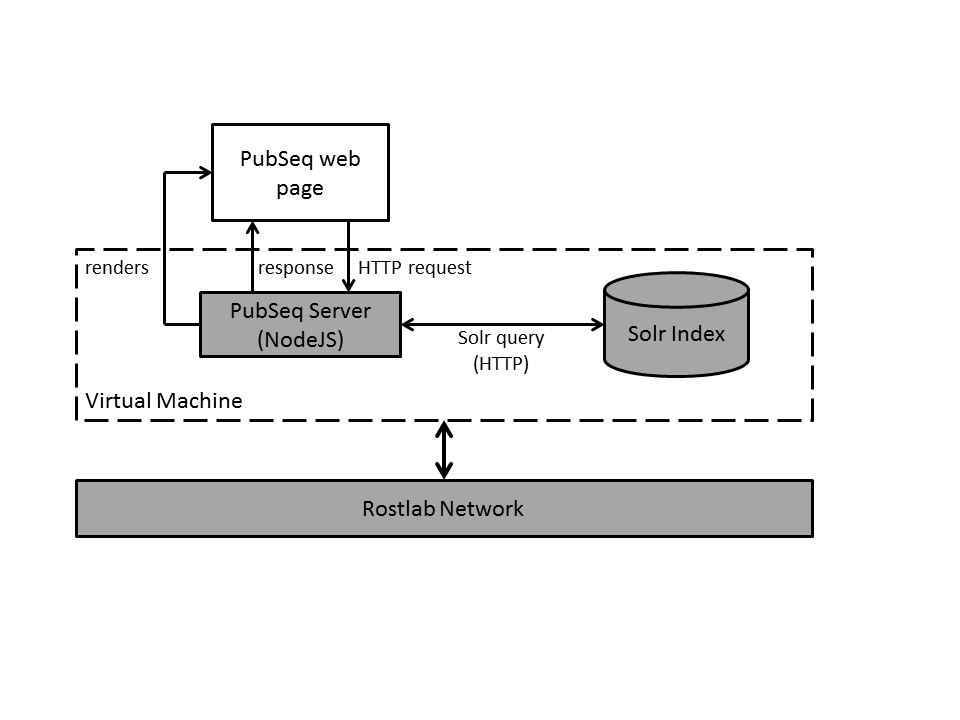
\includegraphics[width=6in]{Figures/pubseq_vm.png}
%    \rule{35em}{0.5pt}
%  \caption[Diagram of the main components of PubSeq with VM parameter highlighted.]{Diagram of the main components of Solr with Virtual Machine environment shown. Here we see that the web page, the only interface between VM and outside world, is isolated from outside world (upper part of the out-of-box area). While a web page could access the Node.js server and Solr index is available everywhere within the Virtual Machine, there is invisible   There are two main modes of index access: query and indexing. Both modes are handled by the top level REST-like service (wrapped in Jetty \citep{jetty}, Tomcat \citep{apachetomcat} or something similar). Each instance consists of multiple core, with each core is defined by configuration files, namely \texttt{solrconfig.xml} (which applies globally across all cores) and \texttt{schema.xml}. Both indexing and query routines would be going through text analysis pipeline for tokenization and other lexical analysis. Solr would then store/fetch several meta-information in/from appropriate Lucene index. Figure adopted from (Grainger, Potter and Seeley, 2014 \citep{grainger2014solr})}
%  \label{fig:SolrComponents}
%\end{figure} 



\label{lst:MEDLINEDTD} 
% Chapter Template

\chapter{PubSeq Web Service} % Main chapter title

\label{Chapter6} % Change X to a consecutive number; for referencing this chapter elsewhere, use \ref{ChapterX}

\lhead{Chapter 6. \emph{PubSeq Web Service}} % Change X to a consecutive number; this is for the header on each page - perhaps a shortened title 
% Chapter Template

\chapter{Conclusions and Outlook} % Main chapter title

\label{Chapter7} % Change X to a consecutive number; for referencing this chapter elsewhere, use \ref{ChapterX}

\lhead{Chapter 7. \emph{Conclusions and Outlook}} % Change X to a consecutive number; this is for the header on each page - perhaps a shortened title
 
% Chapter Template

\chapter{Conclusion and Outlook} % Main chapter title

\label{Chapter8} % Change X to a consecutive number; for referencing this chapter elsewhere, use \ref{ChapterX}

\lhead{Chapter 7. \emph{Conclusion and Outlook}} % Change X to a consecutive number; this is for the header on each page - perhaps a shortened title

In this project we tried to tackle issues arising from two contemporary development in modern bioinformatics:

\begin{itemize}
\item Explosion of the knowledge written information corpus in biomedical research. This is reflecting by the staggering number of publications in biomedical fields which clock at almost 25,000,000 publications at the moment (see previous chapters).

\item Explosion in the number of discovered proteins, especially the automatically annotated non-reviewed proteins.
\end{itemize}

In this project we tried to address the two source of problems seen from the perspective of a human, a researcher. We managed so far to create a working system that address some of the issues posed in Chapter \ref{Chapter1}. Not only working, we design our system to be self-updating especially with more additions of references within MEDLINE corpus. While a perfect portability is practically impossible, we design our Pipeline in a way that it will make extension easier than it would given the system complexity. In administrative side, we also have created an internal developer wiki which would make continuous development possible. Thus we hope that this effort wouldn't stop. And even if it is, we expect the system to keep running and stay updated as we already designed -- this would ensure that our project would stay on helping more researcher in their research later.

Our evaluation shows a promising results with regard to our NER Tagger that we deploy in our system. This is great news since we can be confident that our results are based on robust system. Thus we hope that more researcher could make use of our tool.

The nature of our project means that our system will keep evolving for some time. This would mean that some small things might change or be replaced, for good. We however, we will keep emphasize the importance of both simplicity and intuitive design, particularly regarding our web interface, which will ensure our system usability among broad spectrum of user (from undergraduate students to senior principal investigators). Administratively, we wish to continue this project actively until early part of next year as Master Project. As thus, there would be more updates coming in this project, which we are excited about. 

%----------------------------------------------------------------------------------------
%	THESIS CONTENT - APPENDICES
%----------------------------------------------------------------------------------------

\addtocontents{toc}{\vspace{2em}} % Add a gap in the Contents, for aesthetics

\appendix % Cue to tell LaTeX that the following 'chapters' are Appendices

% Include the appendices of the thesis as separate files from the Appendices folder
% Uncomment the lines as you write the Appendices

% Appendix A

\chapter{PubSeq Paths and Source URLs} % Main appendix title

\label{AppendixA} % For referencing this appendix elsewhere, use \ref{AppendixA}

\lhead{Appendix A. \emph{PubSeq Paths and Source URLs}} % This is for the header on each page - perhaps a shortened title

%----------------------------------------------------------------------------------------
%	SECTION 1
%----------------------------------------------------------------------------------------

\section{Source Codes}

There are several source codes that are relevant to our project:

\begin{itemize}
\item \href{https://rostlab.informatik.tu-muenchen.de/gitlab/gyachdav/pubseq-crawler}{\texttt{https://rostlab.informatik.tu-muenchen.de/gitlab/gyachdav/pubseq-crawler}} contains the tagging ('crawler') pipeline of our project. It also contains several scripts that are used in this project (most notably \texttt{annotate\_new.sh} and \texttt{maintenance.sh}.
\item \href{https://rostlab.informatik.tu-muenchen.de/gitlab/gyachdav/pubseq-frontend}{\texttt{https://rostlab.informatik.tu-muenchen.de/gitlab/gyachdav/pubseq-frontend}} contains the node.js implementation of our project.
\end{itemize}

%----------------------------------------------------------------------------------------
%	SECTION 2
%----------------------------------------------------------------------------------------

\section{Project Location}

Generally the project will be located at \texttt{/mnt/project/pubseq/} within Rostlab server. The directory is further divided into following categories:

\begin{verbatim}
- /mnt/project/pubseq
|- index_input_docs
|- log
|- named_entity_tagger
|- programdata
|- rundata
|- solr_index
|- scripts
|- stats 
\end{verbatim}

The overview of each of directories is as follow:

\begin{itemize}
\item \texttt{index\_input\_docs} contains the files that would be indexed onto Solr. In other words, this directory contains all files that were created during Tagging Pipeline. During the last step of Tagging Pipelines, the program \texttt{SolrUpdater.jar} would point at this directory and index files that match certain pattern of file name.
\item \texttt{log} contains logs from Tagging Pipeline.
\item \texttt{named\_entity\_tagger} contains the \textbf{Lars Tagger component} of the Tagging Pipeline.
\item \texttt{programdata} contains several program-related tab-separated files that would be used and/or produced during the Tagging Pipeline. Note that program-related data is different from run-related data (which are located at \texttt{rundata} in which program-related data remain mostly constant across all runs while run-related data were created during one of the steps within the Tagging Pipeline. 
\item \texttt{rundata} contains interim results from Tagging Pipeline and other Tagging-related data. Since Tagging Pipelines consist of multiple programs with each taking input and writing output, it is inevitable that there would be several interim values. The Tagging Pipeline is designed to write standardized in-between values. While the files would not be removed upon completion of one Tagging Pipeline run, they would be overwritten during the next run. The interim values wouldn't be backed up in some consistent environment.
\item \texttt{solr\_index} contains the Solr directory for the project. For readers who are not familiar with Solr, assuming it as "NoSQL Database" would be sufficient. Solr index is self-contained in the way that the only thing that is needed for it to run properly is its own directory (and JDK).
\item \texttt{scripts} contain scripts that would be run for various purposes. The most essentials of all scripts are the \texttt{annotate\_new.sh} and \texttt{maintenance.sh}. \texttt{annotate\_new.sh} wraps the whole Tagging Pipeline process and calls sequentially each component within the pipeline. \texttt{maintenance.sh} contains the Maintenance Pipeline and like \texttt{annotate\_new.sh} calls each component within Maintenance Pipeline sequentially. Both Tagging and Maintenance Pipelines would be further described in later chapters.
\item \texttt{stats} is deprecated or might not be necessary for the whole process. It contains some descriptive statistics from the last run of Tagging Pipeline. For each Tagging Pipeline, some set of statistic files were created that more or less describe the nature of the run.
\end{itemize}
% Appendix A

\chapter{Figures and Tables} % Main appendix title

\label{AppendixB} % For referencing this appendix elsewhere, use \ref{AppendixA}

\lhead{Appendix B. \emph{Figures and Tables}} % This is for the header on each page - perhaps a shortened title

\begin{sidewaysfigure}[ht]
    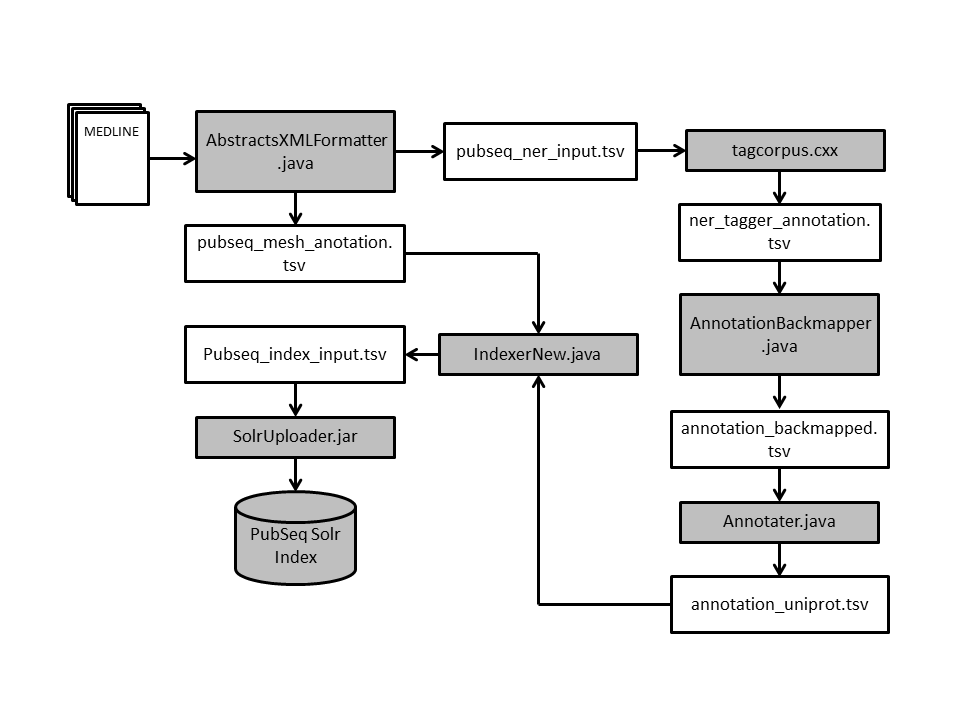
\includegraphics{Figures/tagging_pipeline_complete.png}
    \caption[Overview of PubSeq Tagging Pipeline with all essential programs showed as nodes and important input/output files shown]{Full-sized Overview of PubSeq Tagging Pipeline.}
    \label{fig:PubSeqTaggingFull}
\end{sidewaysfigure}

\begin{figure}

\begin{minipage}{.5\linewidth}
  \centering
  \subfloat[]{\label{AB1:a}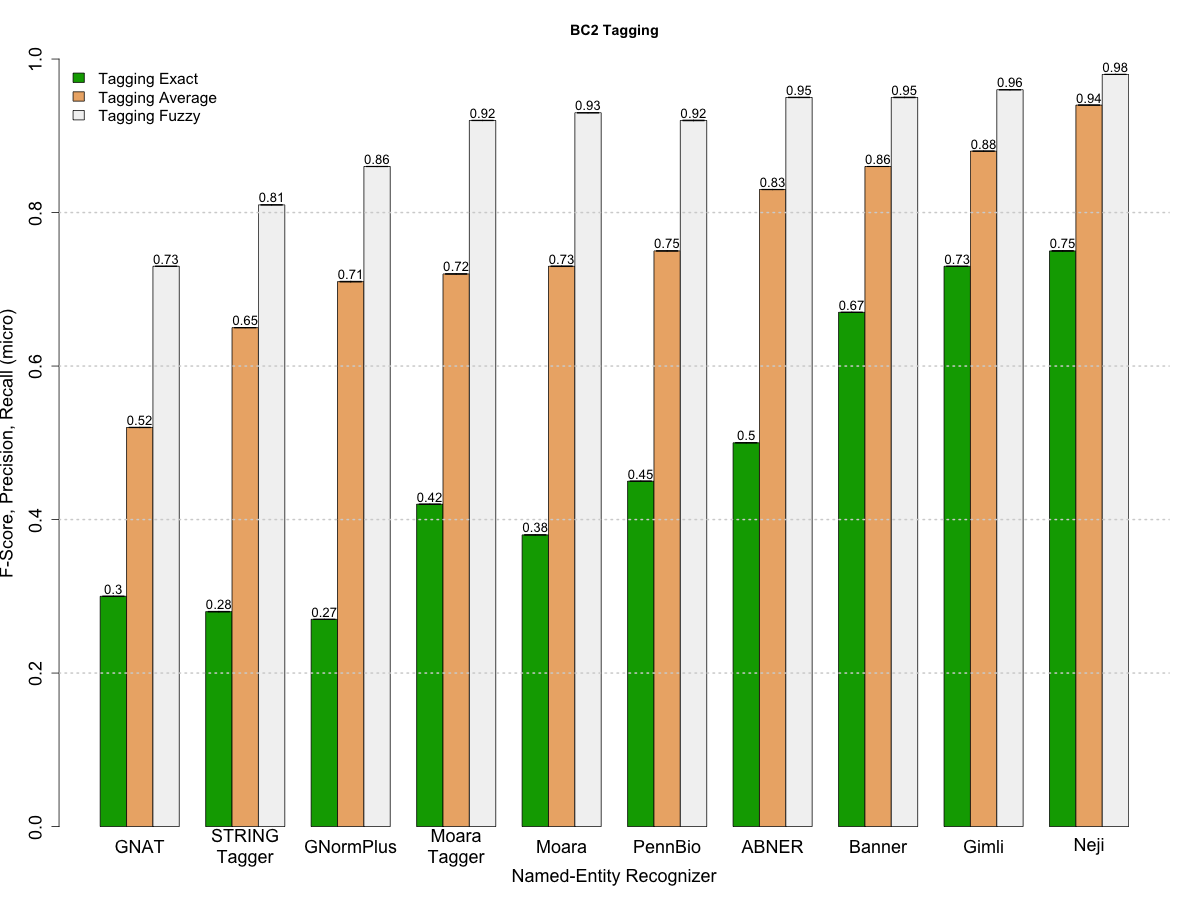
\includegraphics[width=3in]{Figures/eval/appendix/Micro_BC2.png}}
  \end{minipage}%
  \begin{minipage}{.5\linewidth}
  \centering
  \subfloat[]{\label{AB1:b}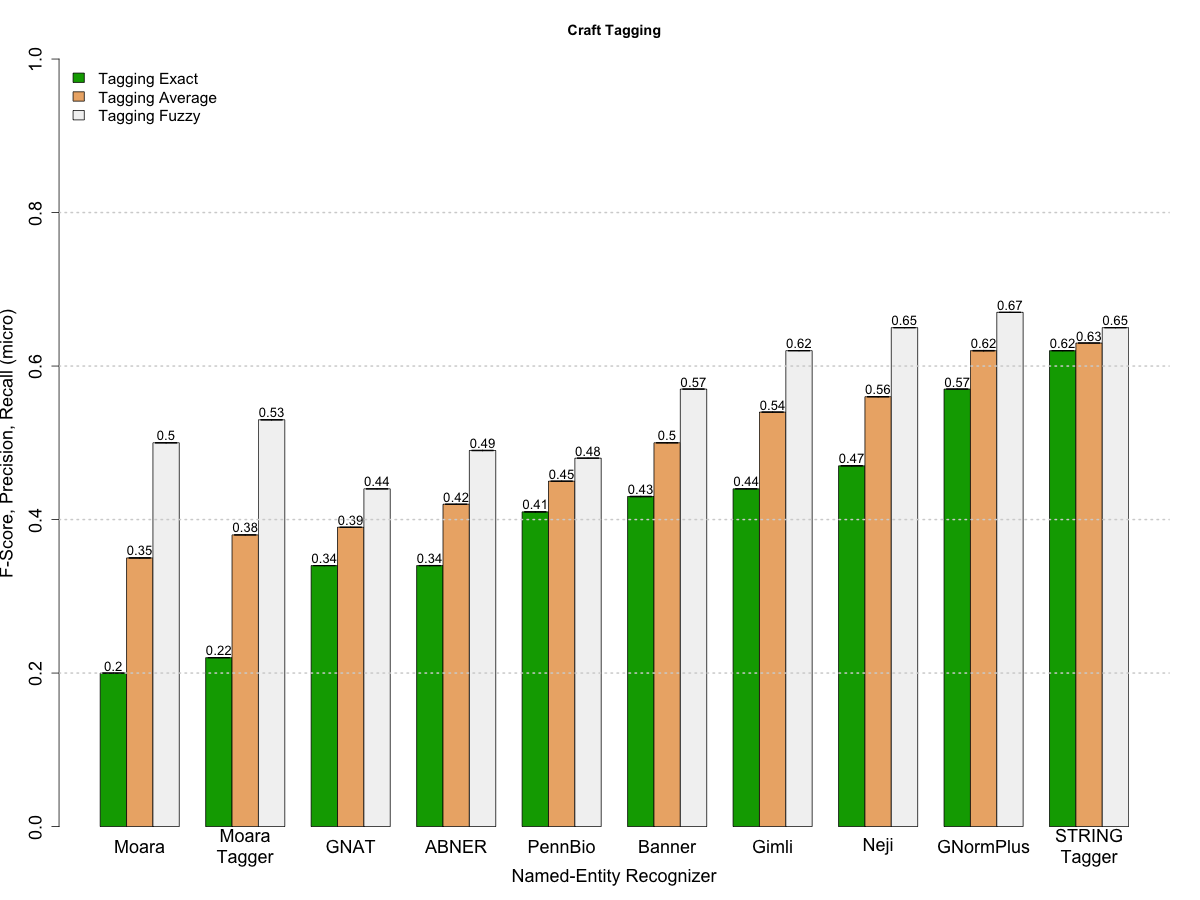
\includegraphics[width=3in]{Figures/eval/appendix/Micro_Craft.png}}
  \end{minipage}\par\medskip
  \begin{minipage}{.5\linewidth}
  \centering
  \subfloat[]{\label{AB1:c}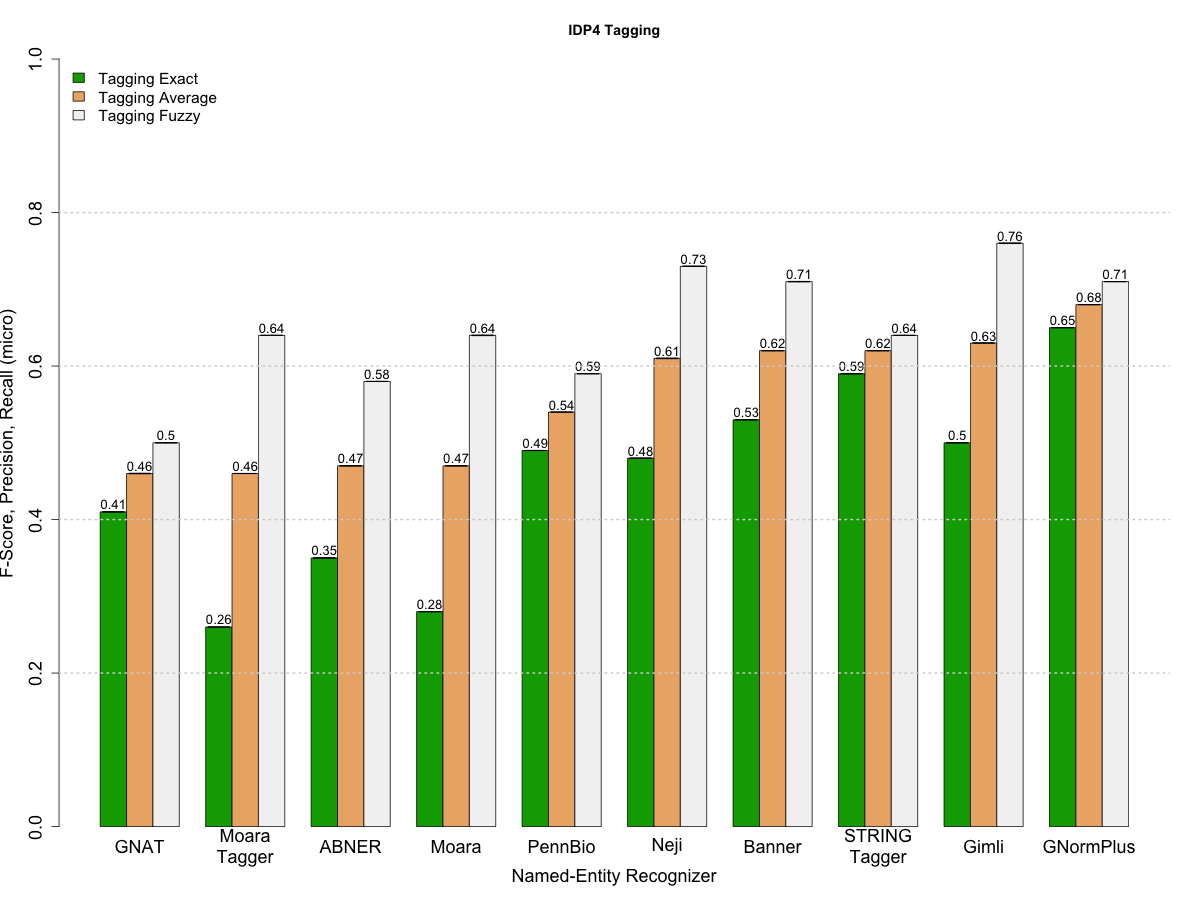
\includegraphics[width=3in]{Figures/eval/appendix/Micro_IDP4.png}}
  \end{minipage}%
  \begin{minipage}{.5\linewidth}
  \centering
  \subfloat[]{\label{AB1:d}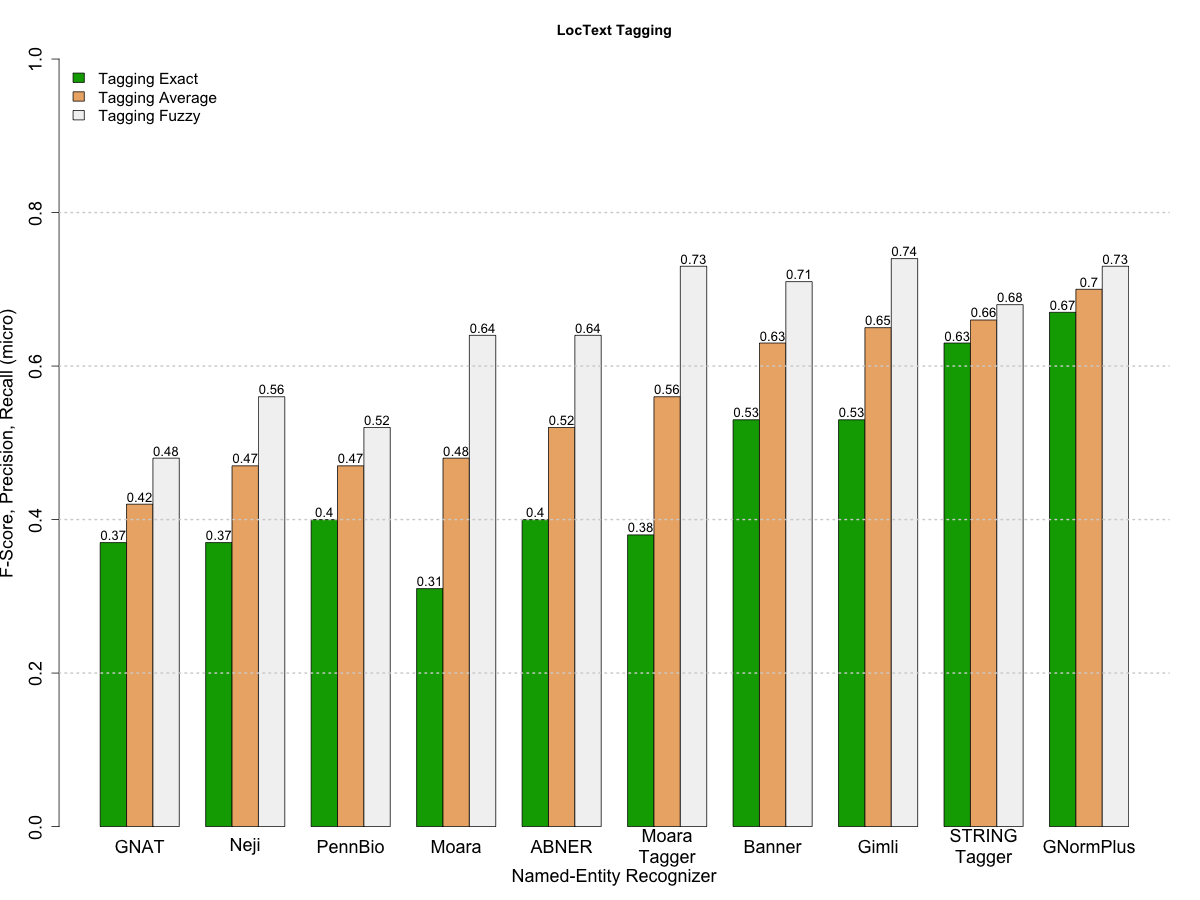
\includegraphics[width=3in]{Figures/eval/appendix/Micro_LocText.png}}
  \end{minipage}\par\medskip

  \caption[Overview of the highest F-Scores in exact, average and fuzzy tagging evaluation]{Overview of detailed F-Scores reached in exact, average and fuzzy tagging, sorted by the score achieved in averaged matching. \ref{AB1:a}: BioCreative II. \ref{AB1:b}: Craft. \ref{AB1:c}: IDP4. \ref{AB1:d} LocText. Adopted from (Ofner, 2015 \citep{ofner2015evaluation})}
\label{fig:AB1}
\end{figure}

\begin{figure}

\begin{minipage}{.5\linewidth}
  \centering
  \subfloat[]{\label{AB2:a}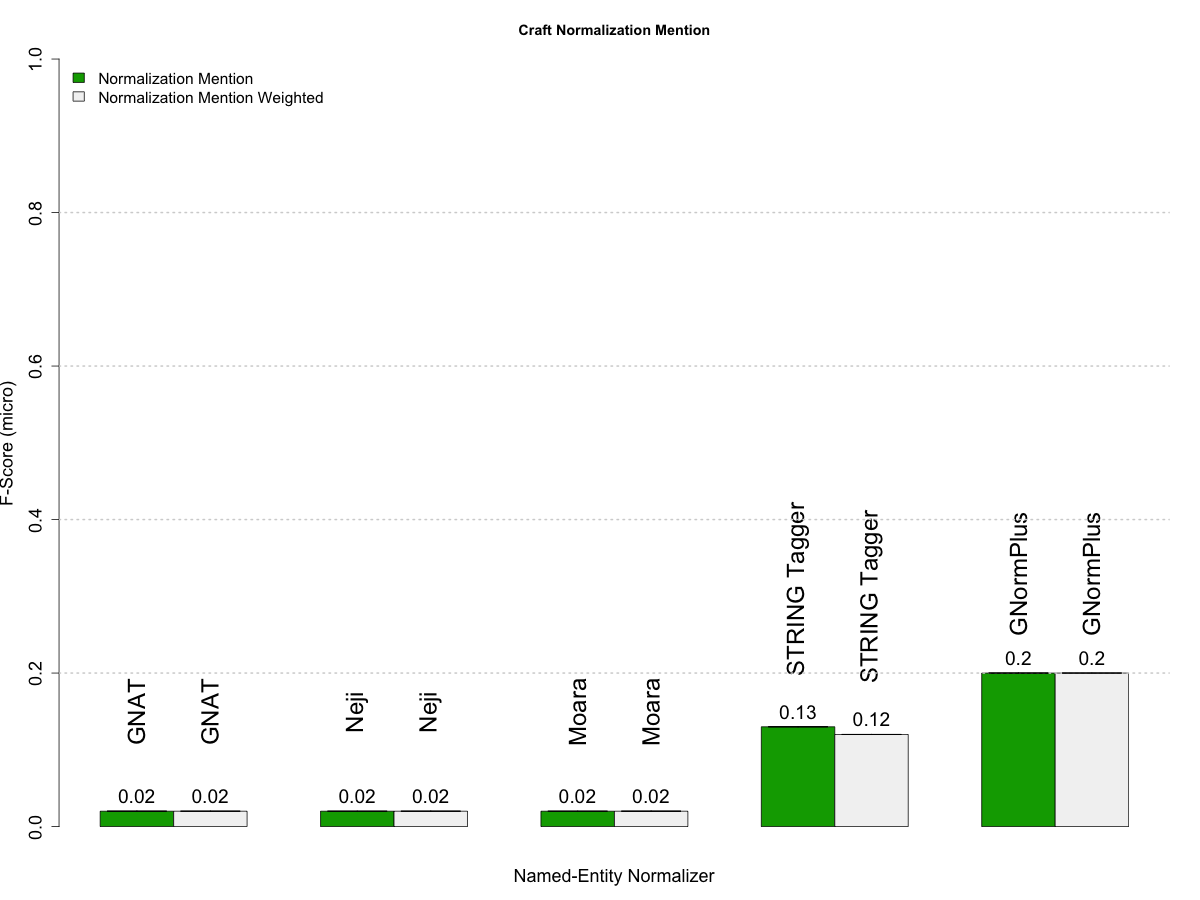
\includegraphics[width=3in]{Figures/eval/appendix/NormalizationMention_Craft.png}}
  \end{minipage}%
  \begin{minipage}{.5\linewidth}
  \centering
  \subfloat[]{\label{AB2:b}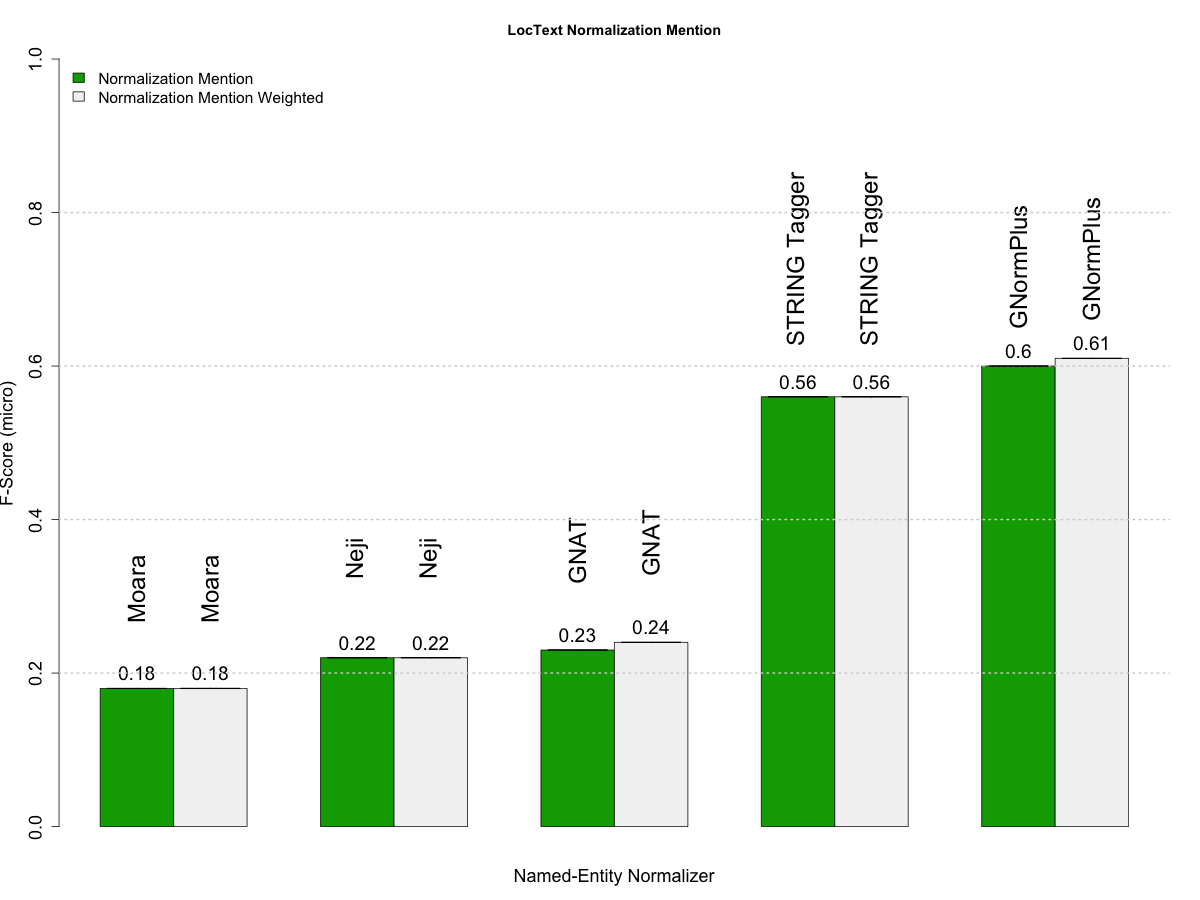
\includegraphics[width=3in]{Figures/eval/appendix/NormalizationMention_LocText.png}}
  \end{minipage}%

  \caption[Overview of detailed F-Scores reached for mention based normalization]{Overview of detailed F-Scores reached for mention based normalization. \ref{AB2:a}: Craft. \ref{AB2:b}: LocText. Adopted from (Ofner, 2015 \citep{ofner2015evaluation})}
\label{fig:AB2}
\end{figure}

\begin{figure}

  \begin{minipage}{.5\linewidth}
  \centering
  \subfloat[]{\label{AB3:a}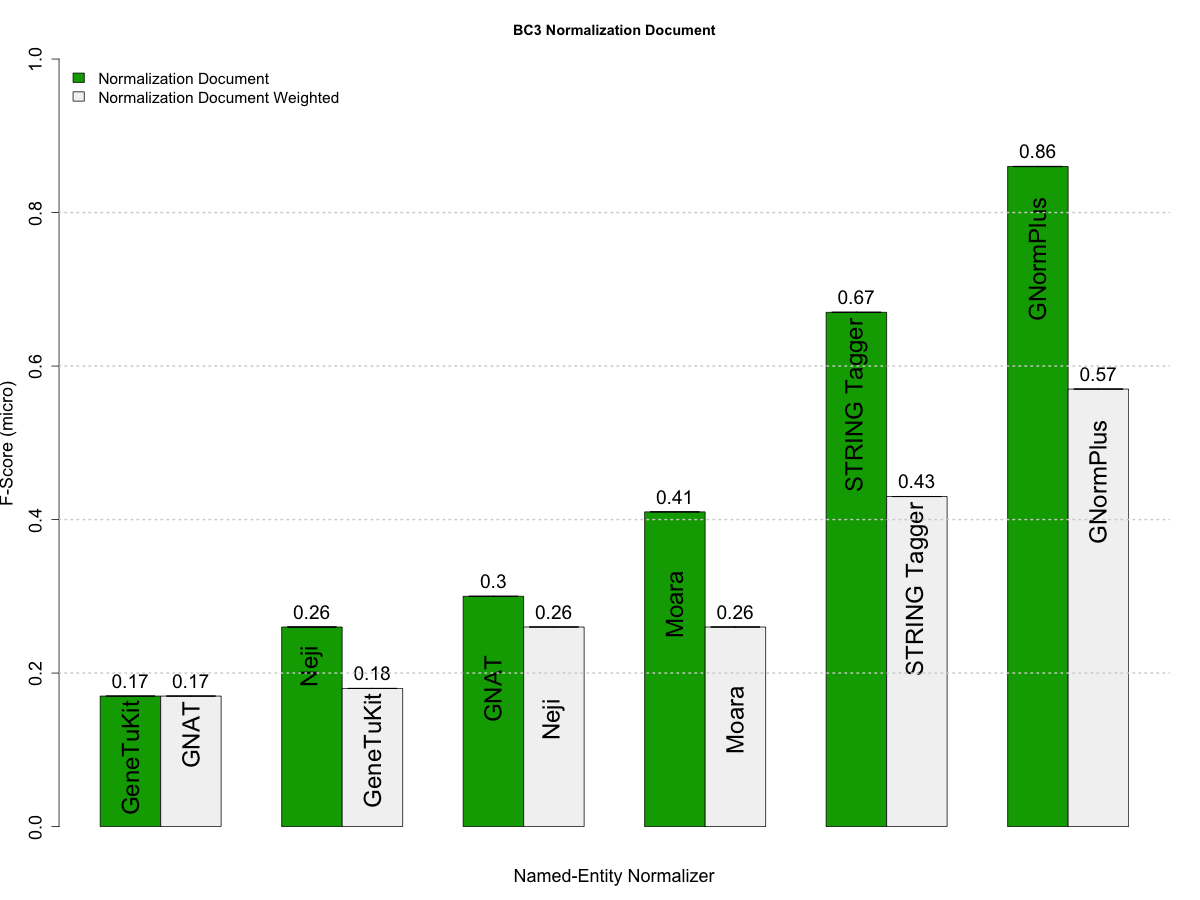
\includegraphics[width=3in]{Figures/eval/appendix/NormalizationDocument_BC3.png}}
  \end{minipage}%
  \begin{minipage}{.5\linewidth}
  \centering
  \subfloat[]{\label{AB3:b}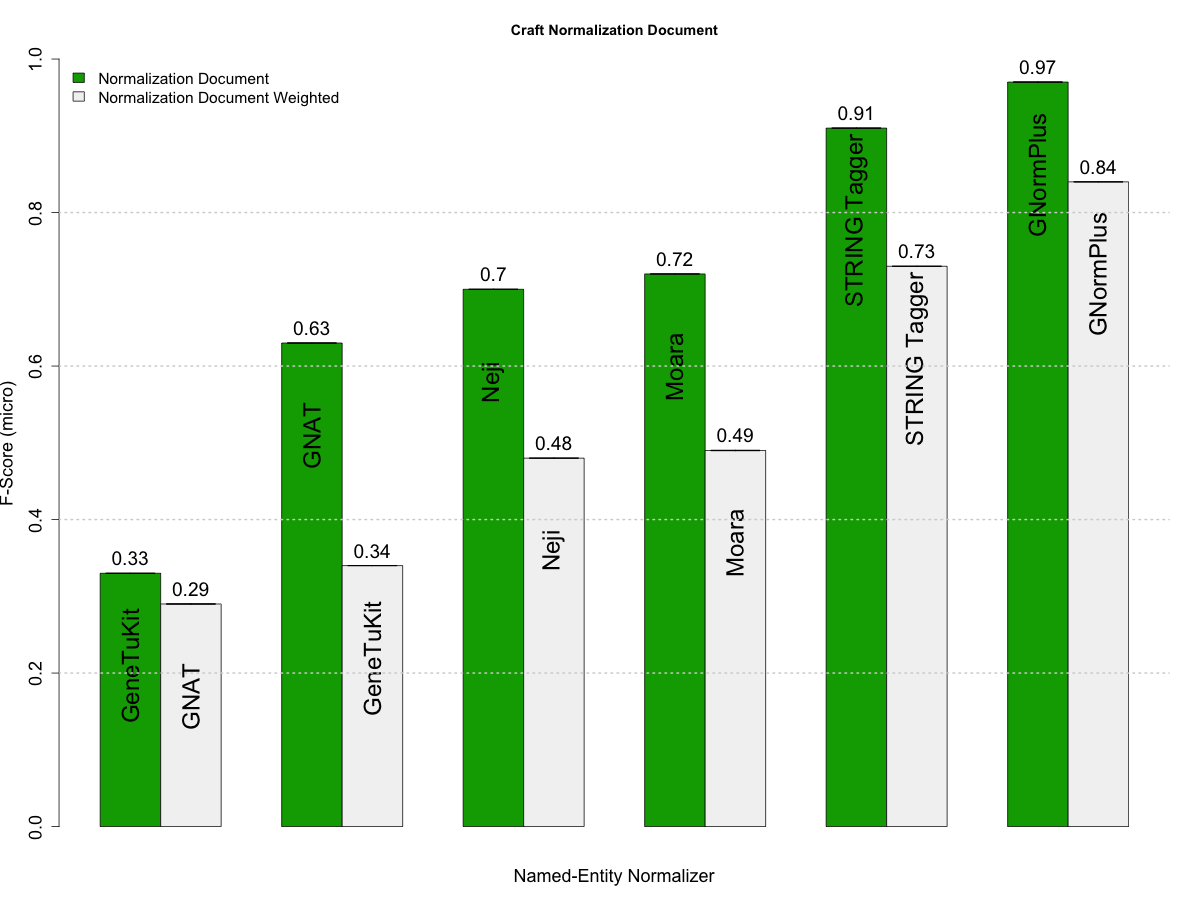
\includegraphics[width=3in]{Figures/eval/appendix/NormalizationDocument_Craft.png}}
  \end{minipage}\par\medskip
  \centering
  \subfloat[]{\label{AB3:c}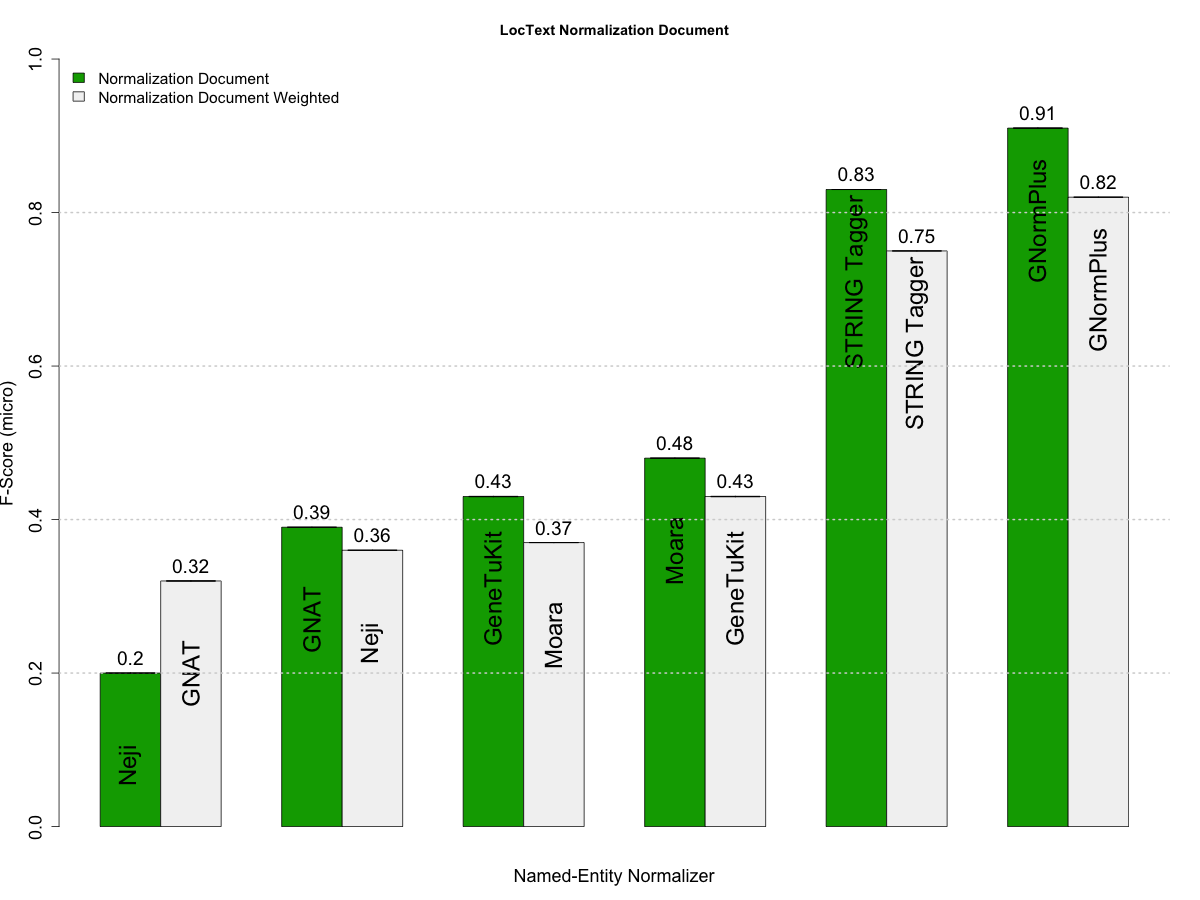
\includegraphics[width=3in]{Figures/eval/appendix/NormalizationDocument_LocText.png}}

  \caption[Overview of detailed F-Scores reached for mention based normalization.
Standard errors are indicated for each F-Score]{Overview of detailed F-Scores reached for mention based normalization. \ref{AB3:a}: BioCreative III. \ref{AB3:b}: Craft. \ref{AB3:c}: LocText. Adopted from (Ofner, 2015 \citep{ofner2015evaluation})}
\label{fig:AB3}
\end{figure}

%\input{Appendices/AppendixC}

\addtocontents{toc}{\vspace{2em}} % Add a gap in the Contents, for aesthetics

\backmatter

%----------------------------------------------------------------------------------------
%	BIBLIOGRAPHY
%----------------------------------------------------------------------------------------

\label{Bibliography}

\lhead{\emph{Bibliography}} % Change the page header to say "Bibliography"

%\bibliographystyle{unsrtnat} % Use the "unsrtnat" BibTeX style for formatting the Bibliography
\bibliographystyle{unsrt}

\bibliography{Bibliography} 

% The references (bibliography) information are stored in the file named "Bibliography.bib"

\end{document}  